\documentclass[12]{article}
\usepackage[utf8]{inputenc}
\usepackage{cite}
\author{par4111 \\ Adrià Cabeza, Xavier Lacasa \\ Departament d' Arquitectura de Computadors}
\title{Lab 1: Experimental setup and tools}
\date{\today \\ 2018 - 19 PRIMAVERA}
\usepackage{graphicx}
\usepackage{subcaption}
\usepackage{pgfplots}
\usepackage{listings}
\usepackage{color}
\usepackage{float}
\definecolor{mauve}{rgb}{0.58,0,0.82}
\definecolor{dkgreen}{rgb}{0,0.6,0}
\lstset{
	frame=tb,language=C,breaklines=true,numbers=none, commentstyle=\color{dkgreen}, stringstyle=\color{mauve}, tabsize=3,   showstringspaces=false,
  columns=flexible, 
}
\begin{document}
\maketitle
\vspace*{\fill}
\begin{center}

\includegraphics[scale=0.5]{images/UPClogo.png}
\end{center}

\newpage
\tableofcontents
\newpage
\section{Introduction}
In order to do properly this subject, first, we have to introduce some new concepts and hardware and software environment that we will use during this semester to do all laboratory assignments.  The following document contains an introductory approach, step by step introducing those concepts. We will introduce the \textit{Boada} architecture, some of the most important parallelism concepts and several tests to see its effects. 

\section{Experimental setup}
\subsection{Node architecture and memory}

\textit{Boada} is a multiprocessor server located at the Computer Architecture Department divided in different nodes, each of them with different architecture and diffferent uses. \textit{Boada} is composed of 8 nodes (from boada-1 to boada-8) and they can be grouped as the following table: 
\\
\begin{table}[h]
\begin{tabular}{|l|l|l|l|}
\hline
Node name    & Processor generation                & Interactive & Queue name \\ \hline
boada-1      & Intel Xeon E5645                    & Yes         & batch      \\
boada-2 to 4 & Intel Xeon E5645                    & No          & execution  \\
boada-5      & Intel Xeon E5-2620 v2 + Nvidia K40c & No          & cuida      \\
boada-6 to 8 & Intel Xeon E5-2609 v4               & No          & execution2 \\ \hline
\end{tabular}
\end{table}

However in this course we are going to use mainly from boada-1 to boada-4. The easiest way to obtain the information of the hardware used in each node is using the linux commands lscpu and lstopo(see Figure  ~\ref{fig:lstopto2} and ~\ref{fig:lstopto8}). This commands can be easily executed in the boada-1 node (because it is interactive), but if we want to use the other nodes we can use the submit-*.sh script provided by the PAR professors and use the queue system. \\
\medskip

\begin{figure}[h]
\centering  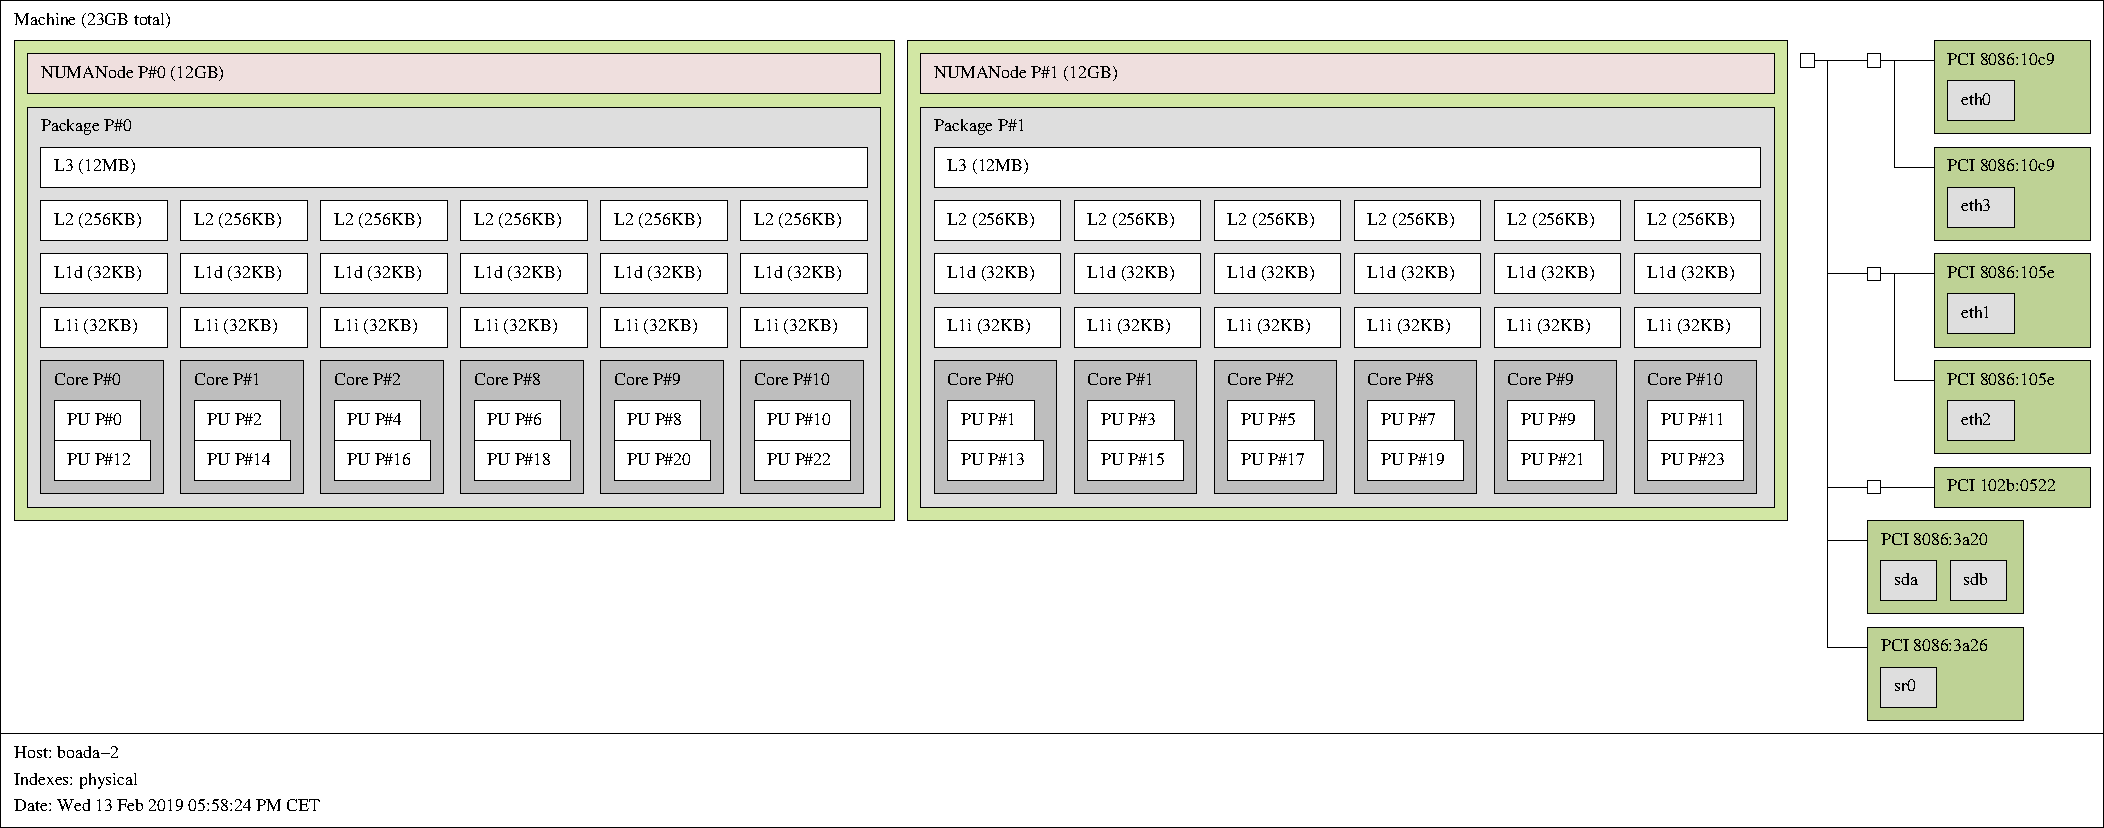
\includegraphics[width=.8\linewidth]{images/map-2.png}
  \caption{Boada-2 architecture outputed by lstopo.}
  \label{fig:lstopto2}
\end{figure}

\begin{figure}[h]
\centering
  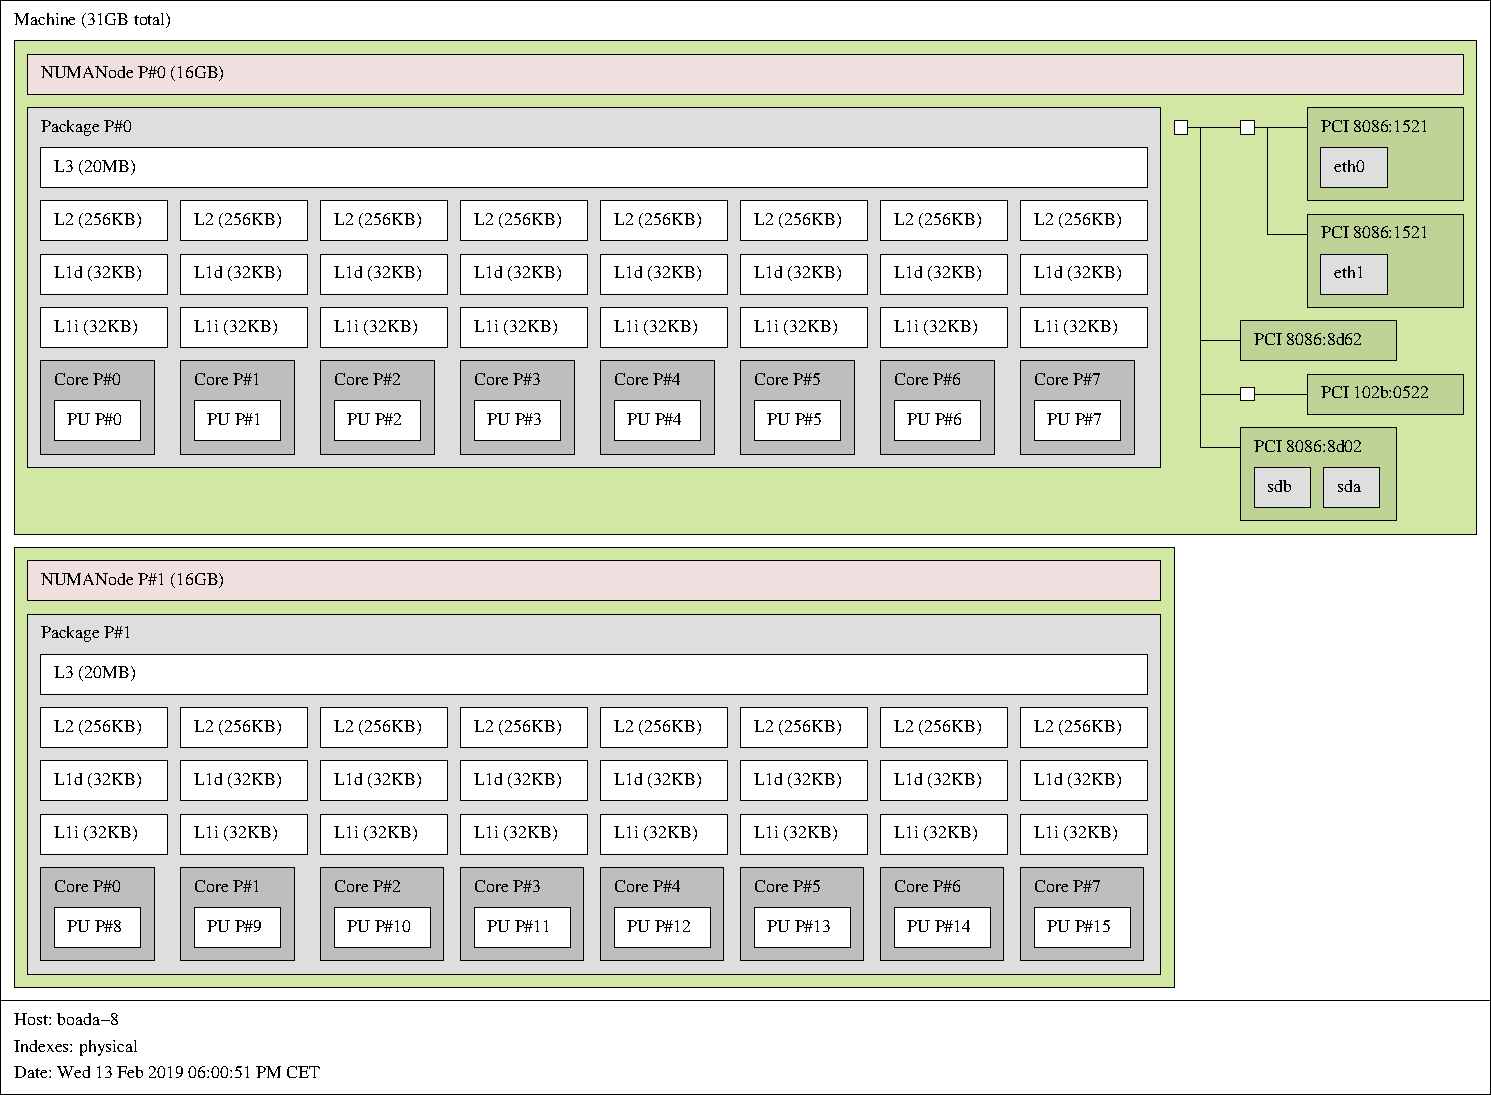
\includegraphics[width=.8\linewidth]{images/map-8.png}
  \caption{Boada-8 architecture outputed by lstopo.}
  \label{fig:lstopto8}
\end{figure}

After creating the scripts and applying them to each of the nodes, we obtained the following hardware information: 


\begin{table}[h]
\centering    \begin{tabular}{|l||l|l|l|}
    \hline
                                        & boada-1 to boada-4    & boada-5   & boada-6 to boada-8    \\
    \hline\hline
    Number of sockets per node          & 2                     & 2         & 2                     \\
    \hline
    Number of cores per socket          & 6                     & 6         & 8                     \\
    \hline
    Number of threads per core          & 2                     & 2         & 1                     \\
    \hline
    L1-I cache size (per-core)          & 32 KB                 & 32 KB     & 32 KB                 \\    
    \hline
    L1-D cache size (per core)          & 32 KB                 & 32 KB     & 32 KB                 \\
    \hline
    L2 cache size (per-core)            & 256 KB                & 256 KB    & 256 KB                \\
    \hline
    Last-level cache size (per-socket)  & 12 MB                 & 15 MB     & 20 MB                 \\
    \hline
    Main memory  size (per socket)      & 12 GB                 & 31 GB     & 16 GB                 \\
    \hline
    Main memory size (per node)         & 23 GB                 & 63 GB     & 31 GB                 \\
    \hline
    \end{tabular}
\end{table}

\bigskip

The previous table gives us useful information that will be necessary in the future to properly use the \textit{boada} system and understand the parallelism decomposition and time we will get. 

\subsection{Sequential and parallel executions}

More often than not parallelism offers speed-ups in the execution time of applications. Sometimes, however, that extra speed is used to augment the problem size, which would not be possible otherwise.

In the two following sections we are going to see the differences of two different approaches to parallelism, \textbf{strong} and \textbf{weak}, applied to the \textit{pi\_omp.c} program.

\subsubsection{Strong scalability}

Strong scalabilty consists in increasing the numberer of processors while keeping the problem size the same. This reduces the amount of work each processor has to do, which speeds-up the execution.
Nonetheless, the speed-up is bounded by the parallelization of the program and the overhead generated when doing so. Usually a point is reached where adding processors has no further effect on the program or the overhead generated by further parallelizing the program is greater than the added speed-up. 

\paragraph{Boada 1:}
For Boada 1 we can see how execution time is logarithmically reduced in Figure \ref{fig:pi_strong_ompboada1}. At 11 threads the time seems to slightly increase. To be sure we can look at the speed-up plot, where we can clearly appreciate how speed-up slowly stops increasing and starts to fall down at around 11 threads. This evidence supports the previous statement about time. This is most likely caused by the overhead that parallelizing a program creates: creating new threads, synchronizing the results, etc. The graphic shows how running the program on 12 threads is actually slower than doing so on 11, and even though we cannot see it in the plots, performance would probably keep going down due to the added overhead with each new thread used.
\begin{figure}[H]
\centering
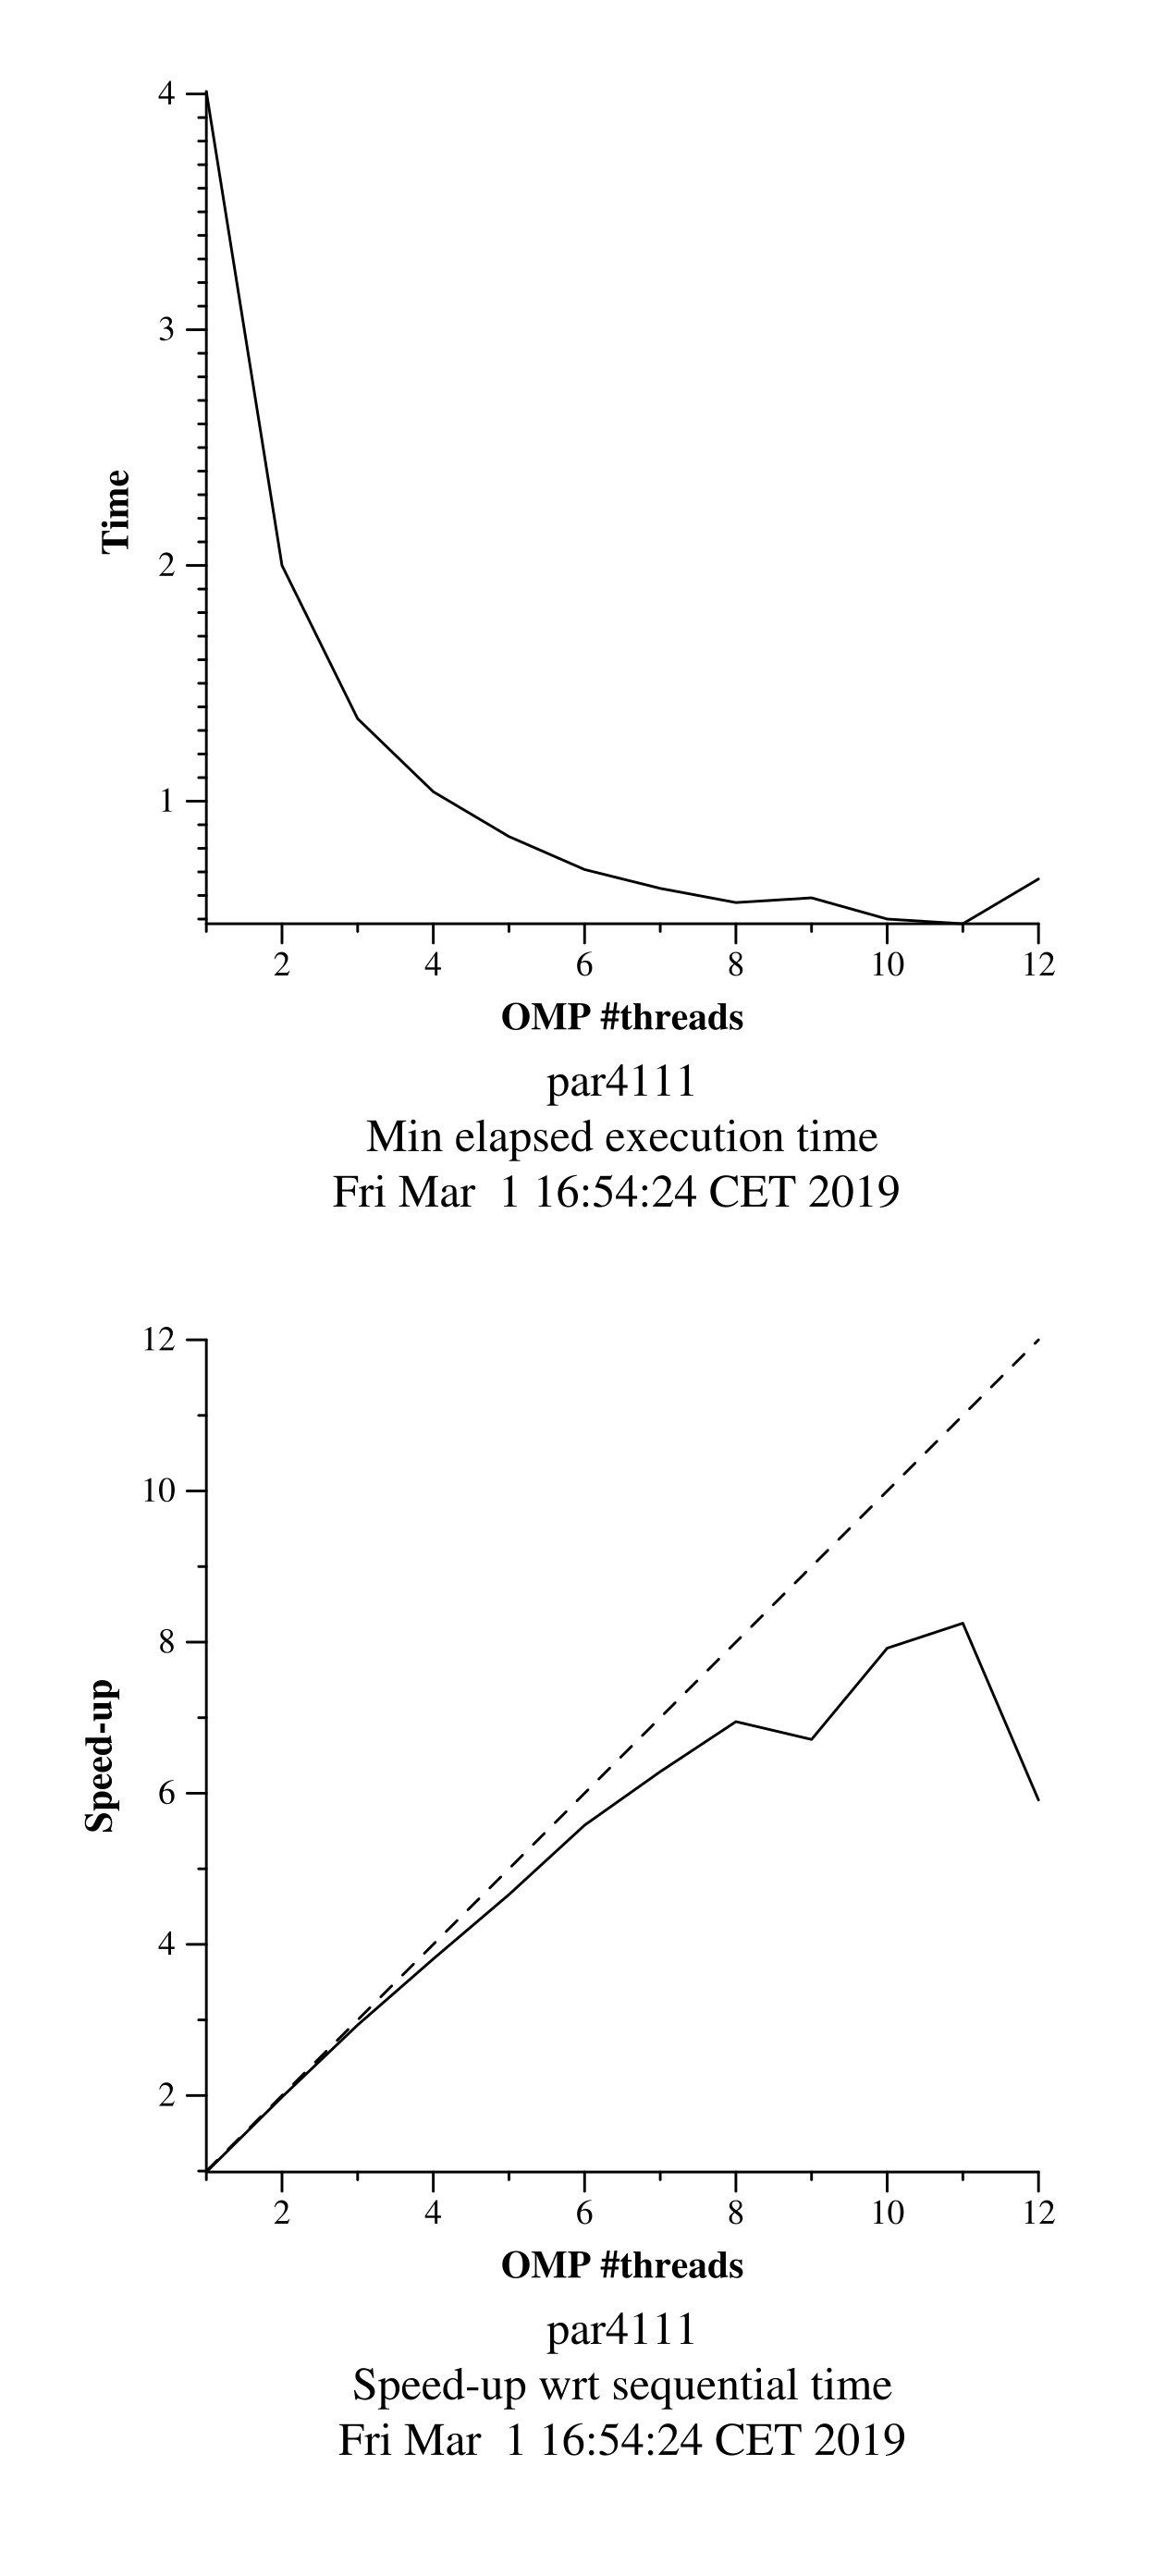
\includegraphics[scale=0.15]{images/pi_omp-1000000000-1-12-3-strong-boada-1.png}
 \caption{ \textit{pi\_omp} with strong scalability by Boada-1}
  \label{fig:pi_strong_ompboada1}
\end{figure}

\bigskip
\paragraph{Boada 2 to 4:}
Since Boada 1 has the same architecture as 2, 3 and 4, it is fair to expect a very similar performance, and in fact that is what Figure \ref{fig:pi_strong_ompboada4} shows. However, Boada 4 speed-up does not quite decrease from using 11 threads to 12, although it certainly does from 10 to 11. Again, it would probably keep decreasing from that point on due to the overhead, but there is an important improvement up until around 10 threads. \\


It would be fair to say that for the \textit{pi\_omp.c} program running Boada 1 to 4, up to 10 threads are beneficial to reduce execution time, but at around 5 threads speed-up starts to increase more slowly at what seems like a logarithmic rate.
\begin{figure}[H]
\centering
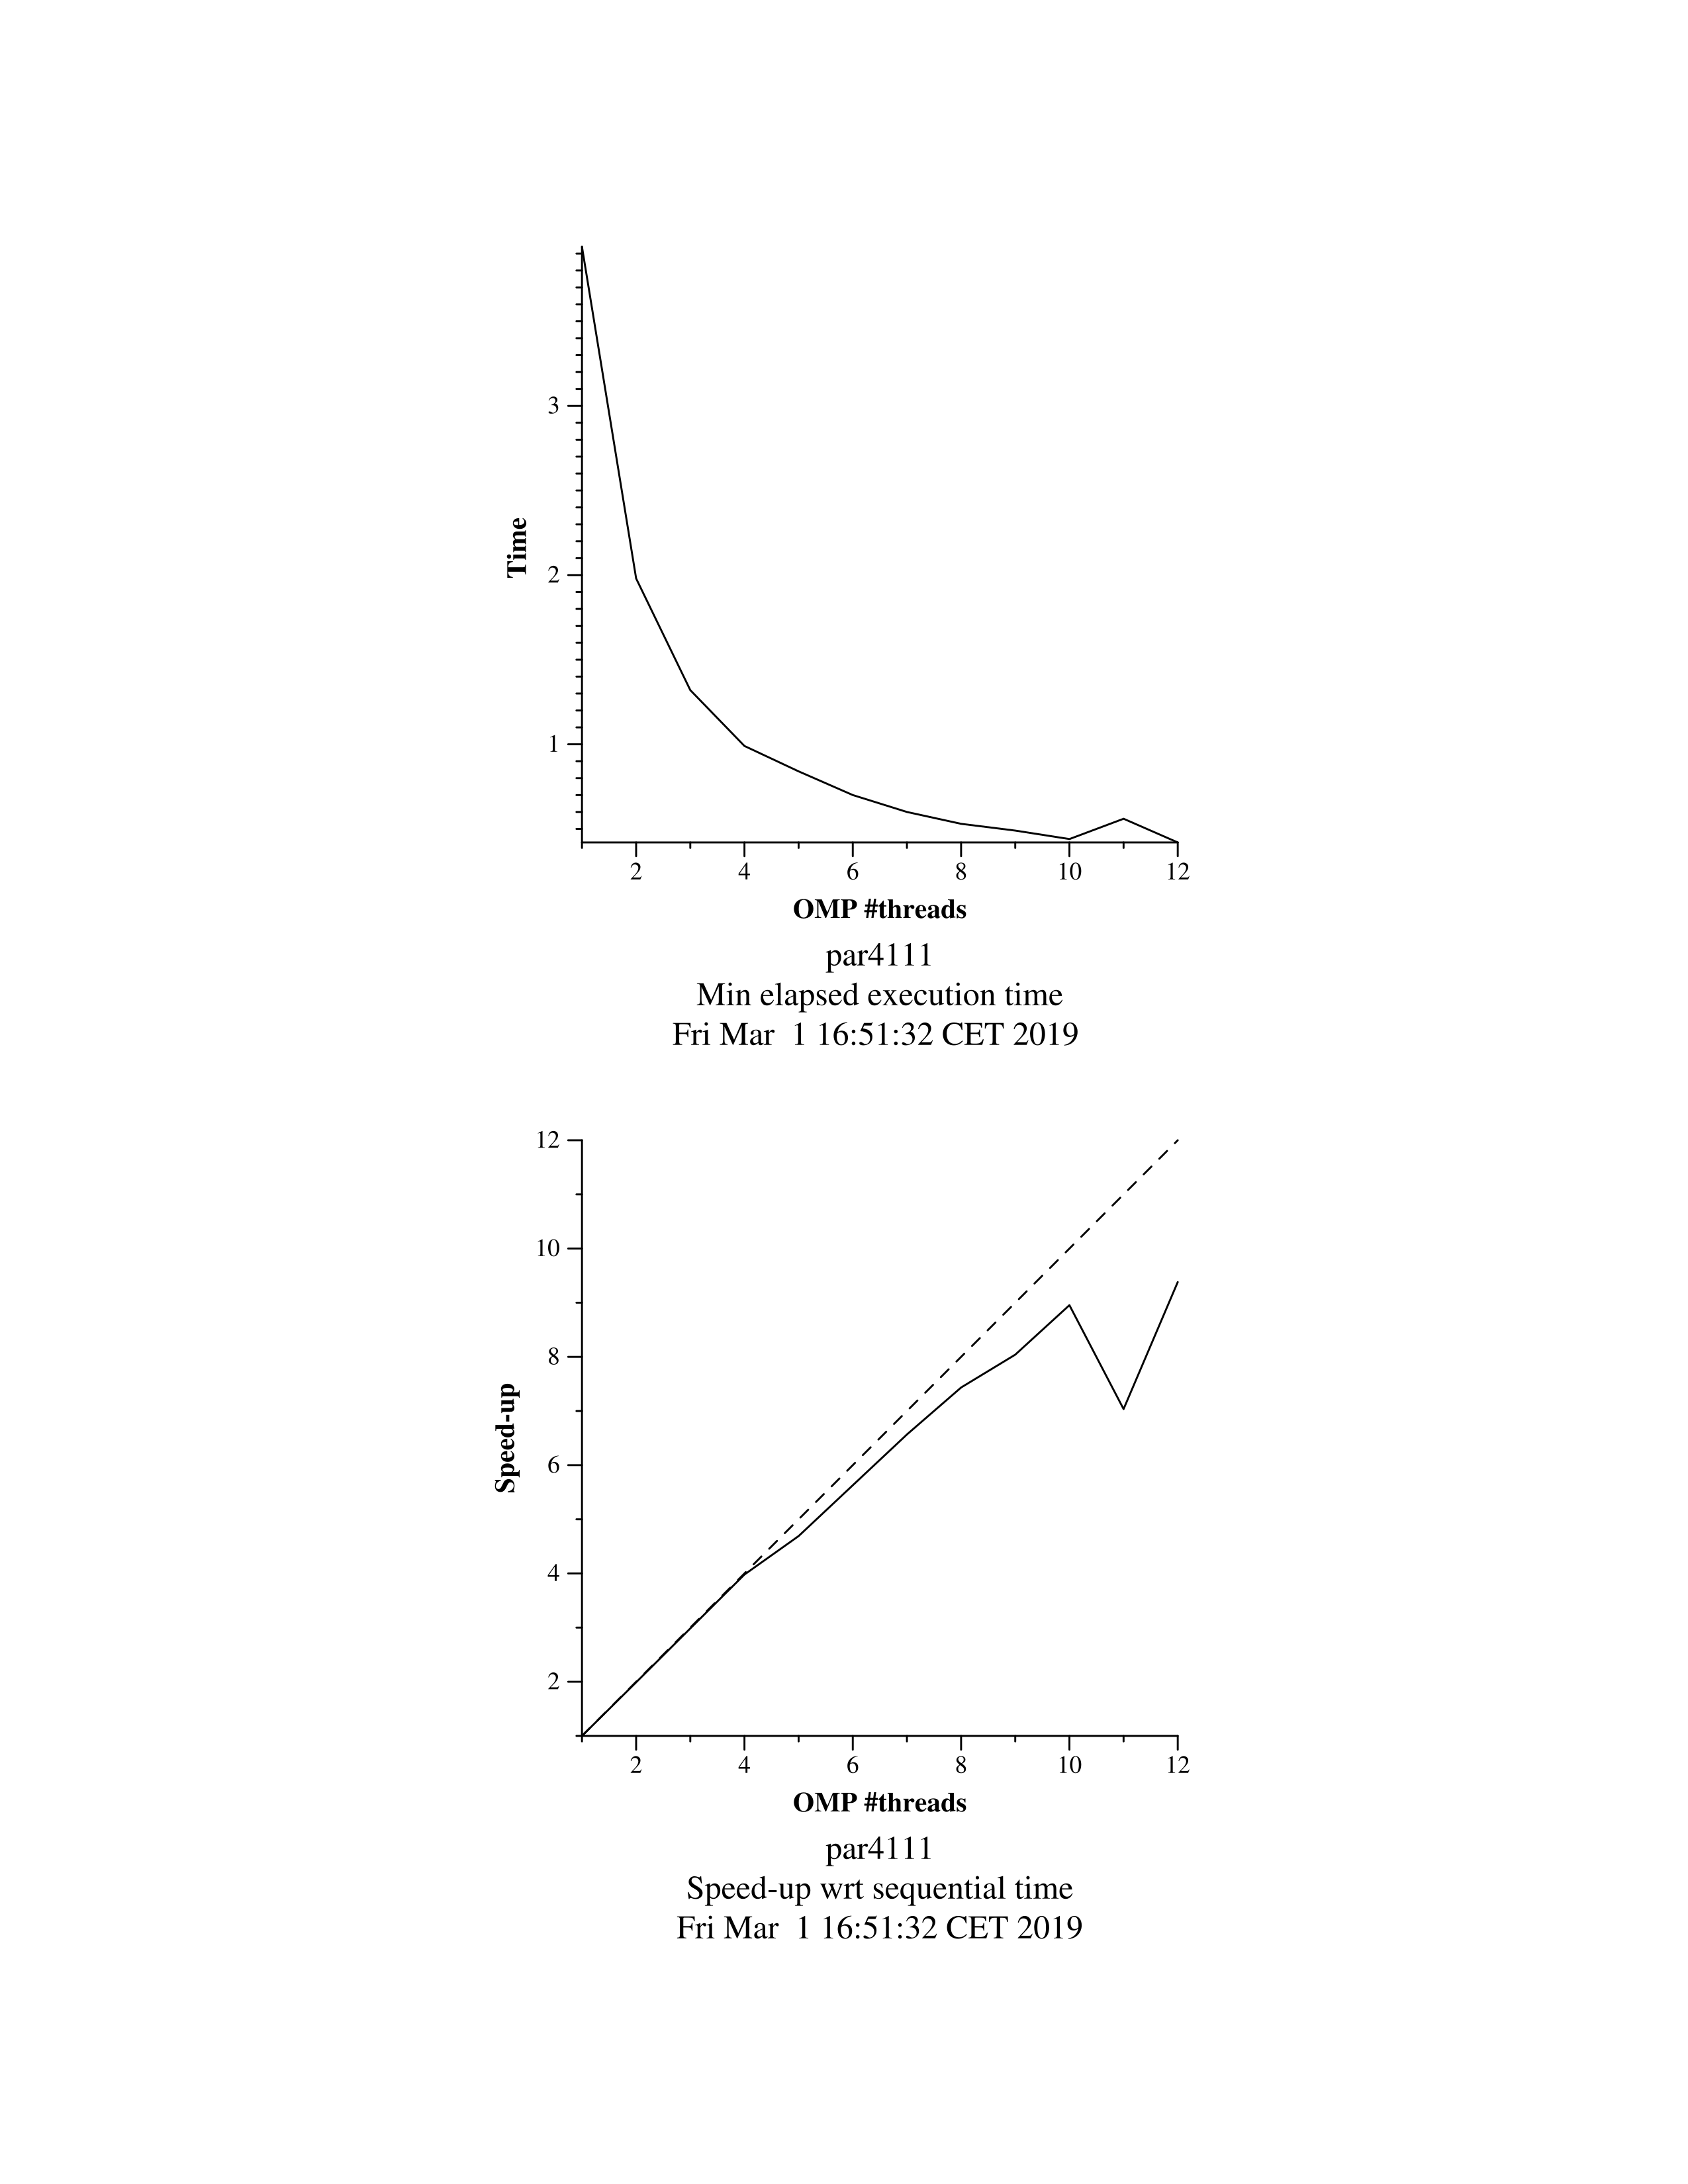
\includegraphics[scale=0.15]{images/pi_omp-1000000000-1-12-3-strong-boada-4.png}
 \caption{ \textit{pi\_omp} with strong scalability by Boada-4}
  \label{fig:pi_strong_ompboada4}
\end{figure}

\bigskip
\paragraph{Boada 5:}
Boada 5 uses a different processor, but the overhead principle should still be present because the generated overhead will start to overcome the parallelization speed-up at some point. In fact, looking at the generated graphics, the loss begins at approximately the same number of threads than the previous Boadas (1-4).  
\begin{figure}[H]
\centering
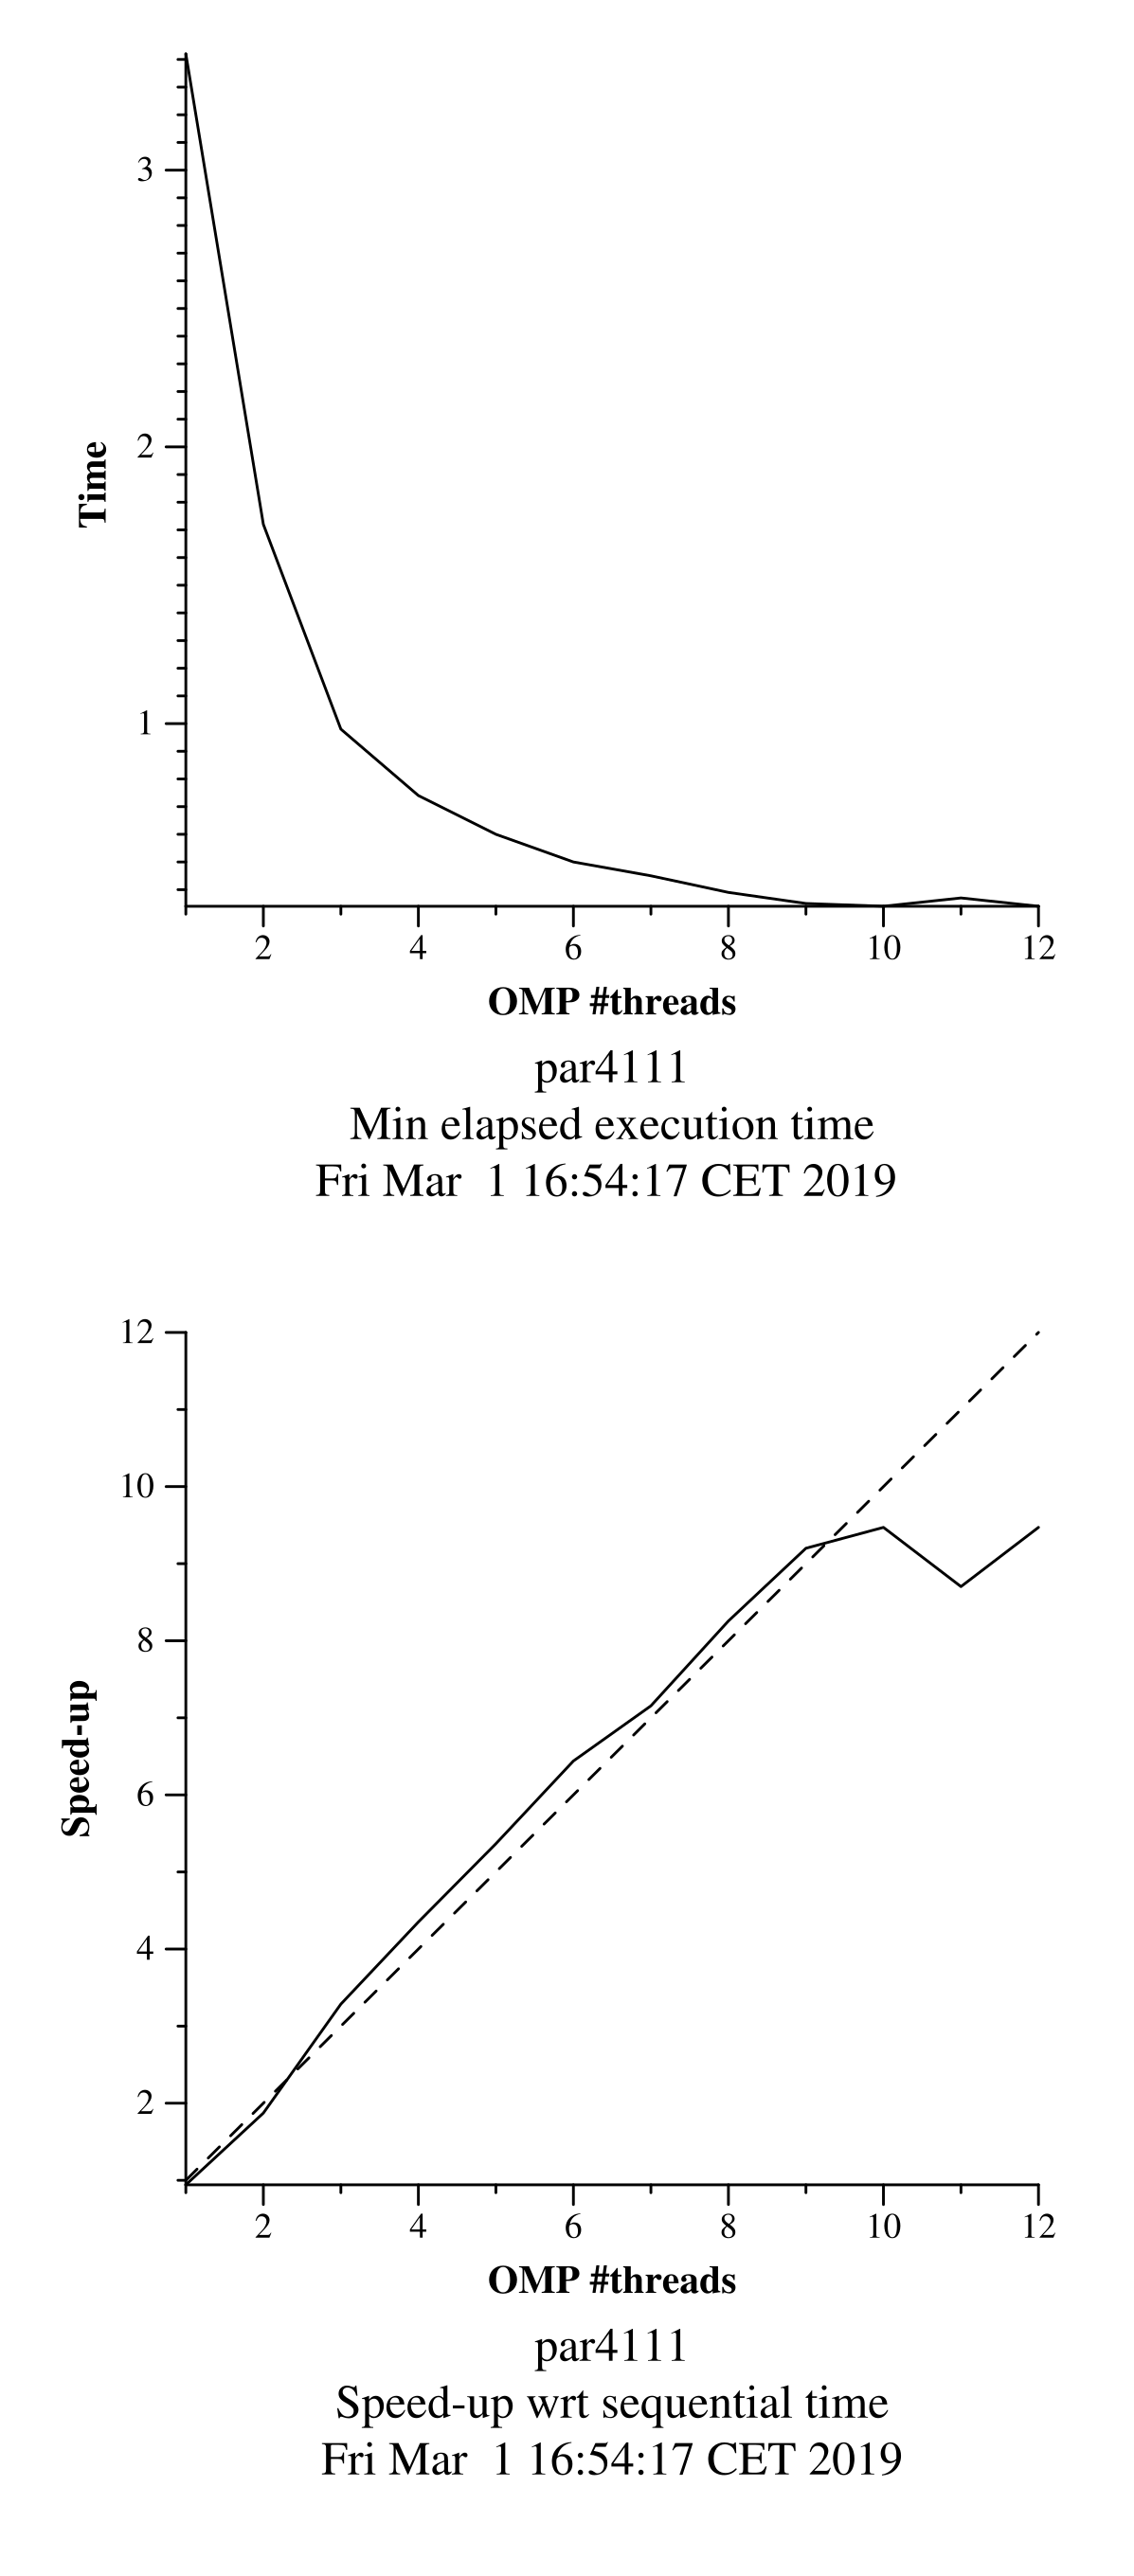
\includegraphics[scale=0.15]{images/pi_omp-1000000000-1-12-3-strong-boada-5.png}
 \caption{ \textit{pi\_omp} with strong scalability by Boada-5}
  \label{fig:pi_strong_ompboada5}
\end{figure}

\bigskip
\paragraph{Boada 6 to 8:}
Boada 6 to 8 use again a different processor. This time, however, the speed-up and time plots look quite different from the previous ones. There is no appreciable decrease in speed-up even up to 12 threads. We speculate that this could be of their processors being newer (Boada 6-8 have Intel Xeon E5-2609 v4), which according to Intel's website have a newer instruction set (Intel® AVX2) and Intel® Transactional Synchronization Extensions New Instructions, which make parallel operations more efficient. Again, we are not sure, it is just a possibility we came up with after doing some research about each Boada's processor architecture. \\
Nevertheless, speed-up should still decay later on if we kept increasing the number of threads, because a point will be reached where the added overhead will surpass the time-reduction gained by parallelism.
\begin{figure}[H]
\centering
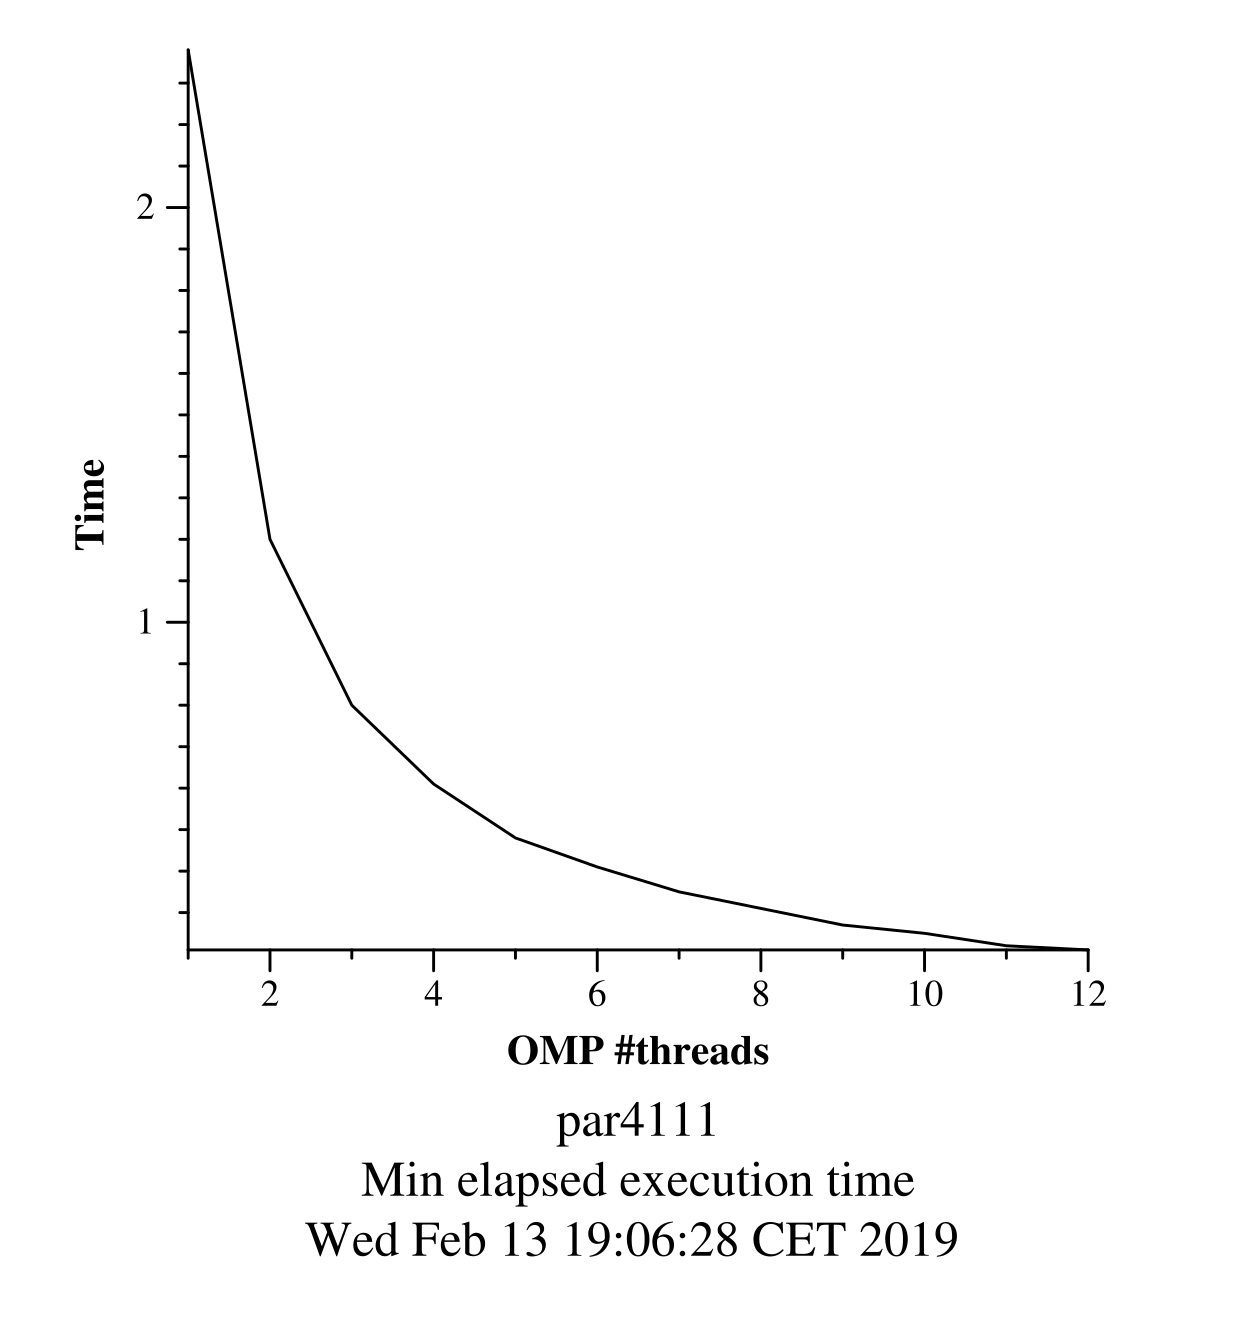
\includegraphics[scale=0.15]{images/pi_omp-1000000000-1-12-3-strong-boada-8.png}
 \caption{ \textit{pi\_omp} with strong scalability by Boada-8}
  \label{fig:pi_strong_ompboada8}
\end{figure}


\bigskip
\subsubsection{Weak scalability}
\paragraph{}

Weak scalability takes a different approach. It takes advantage of the additional power gained by parallelizing the program to increase the problem size proportionally to the number of threads, so that while the speed-up stays more or less the same, the work done increases.

\paragraph{Boada 1:}
For Boada 1 with weak scalability the graphic clearly shows how speed-up stays mostly the same at first. This is due to increasing the problem size proportionally to the number of threads. At around 9 threads, however, the speed-ups starts to decrease similarly to strong scalability. The reason is the same: excess overhead created by parallelization. To keep speed-up the same from this point on we should start to increase the problem size more slowly while keeping the thread number increment the same. 
\begin{figure}[H]
\centering
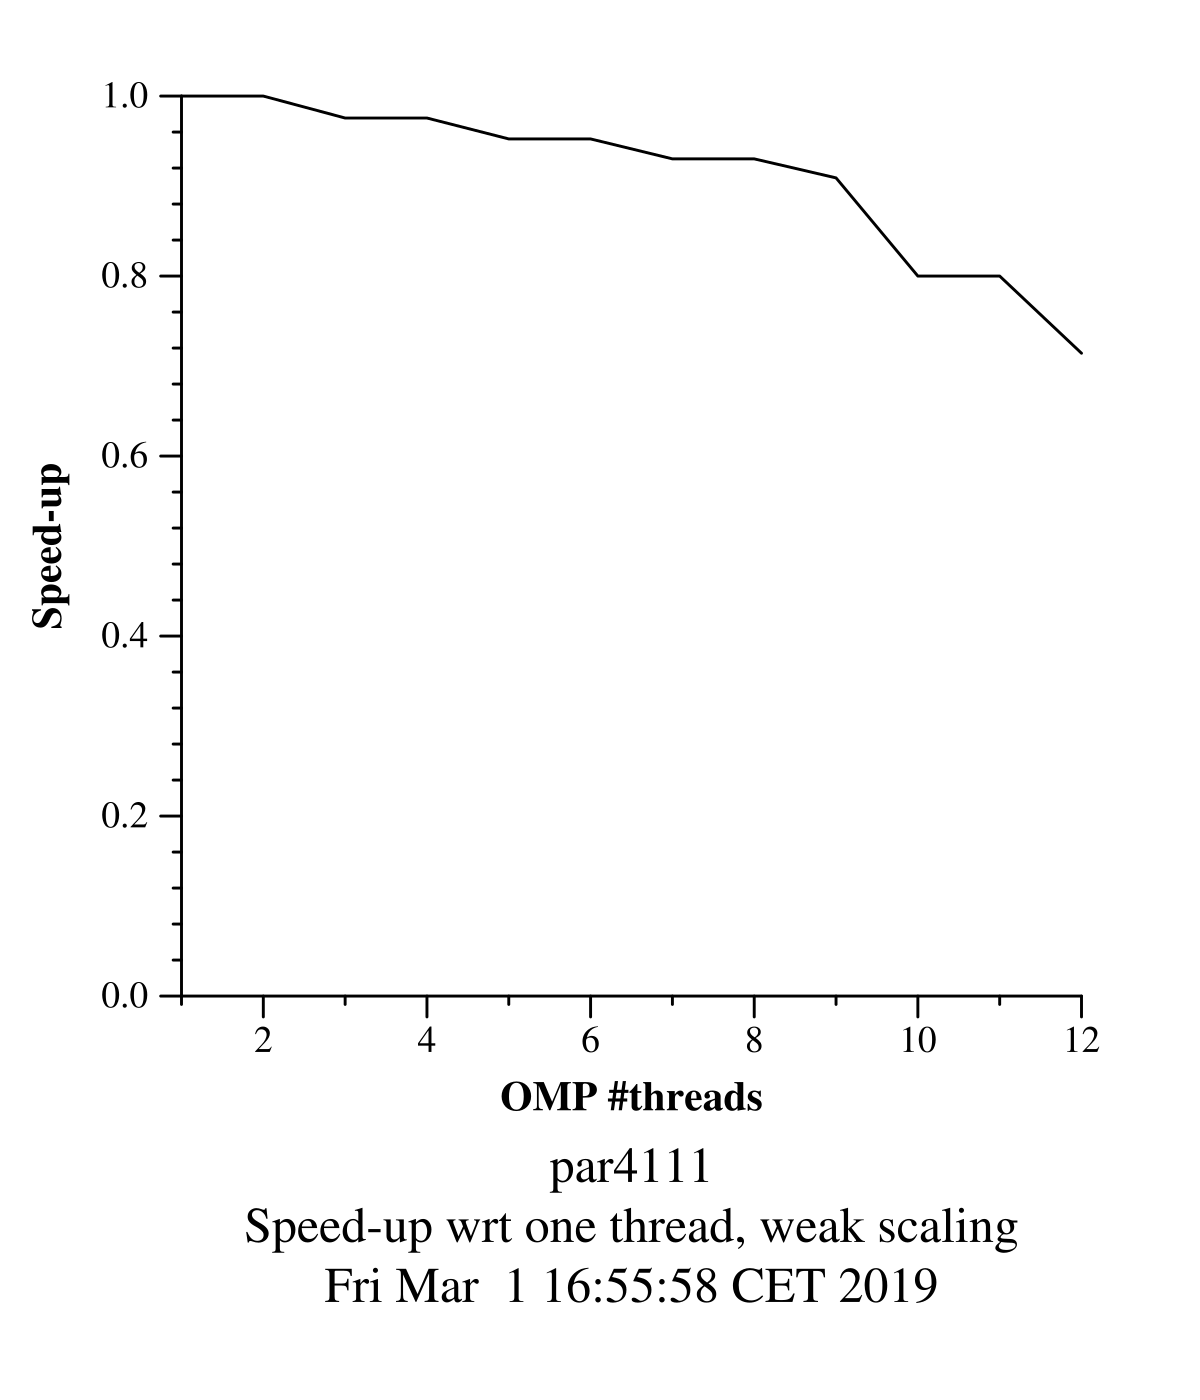
\includegraphics[scale=0.15]{images/pi_omp-100000000-1-12-3-weak-boada-1.png}
 \caption{ \textit{pi\_omp} with weak scalability by Boada-1}
  \label{fig:pi_weak_ompboada1}
\end{figure}

\bigskip
\paragraph{Boada 2 to 4:}
As with strong scalability, Boada 2 to 4 produce a very similar result to Boada 1 due to them having the same processor. There is not much to add with respect to Boada 1.
\begin{figure}[H]
\centering
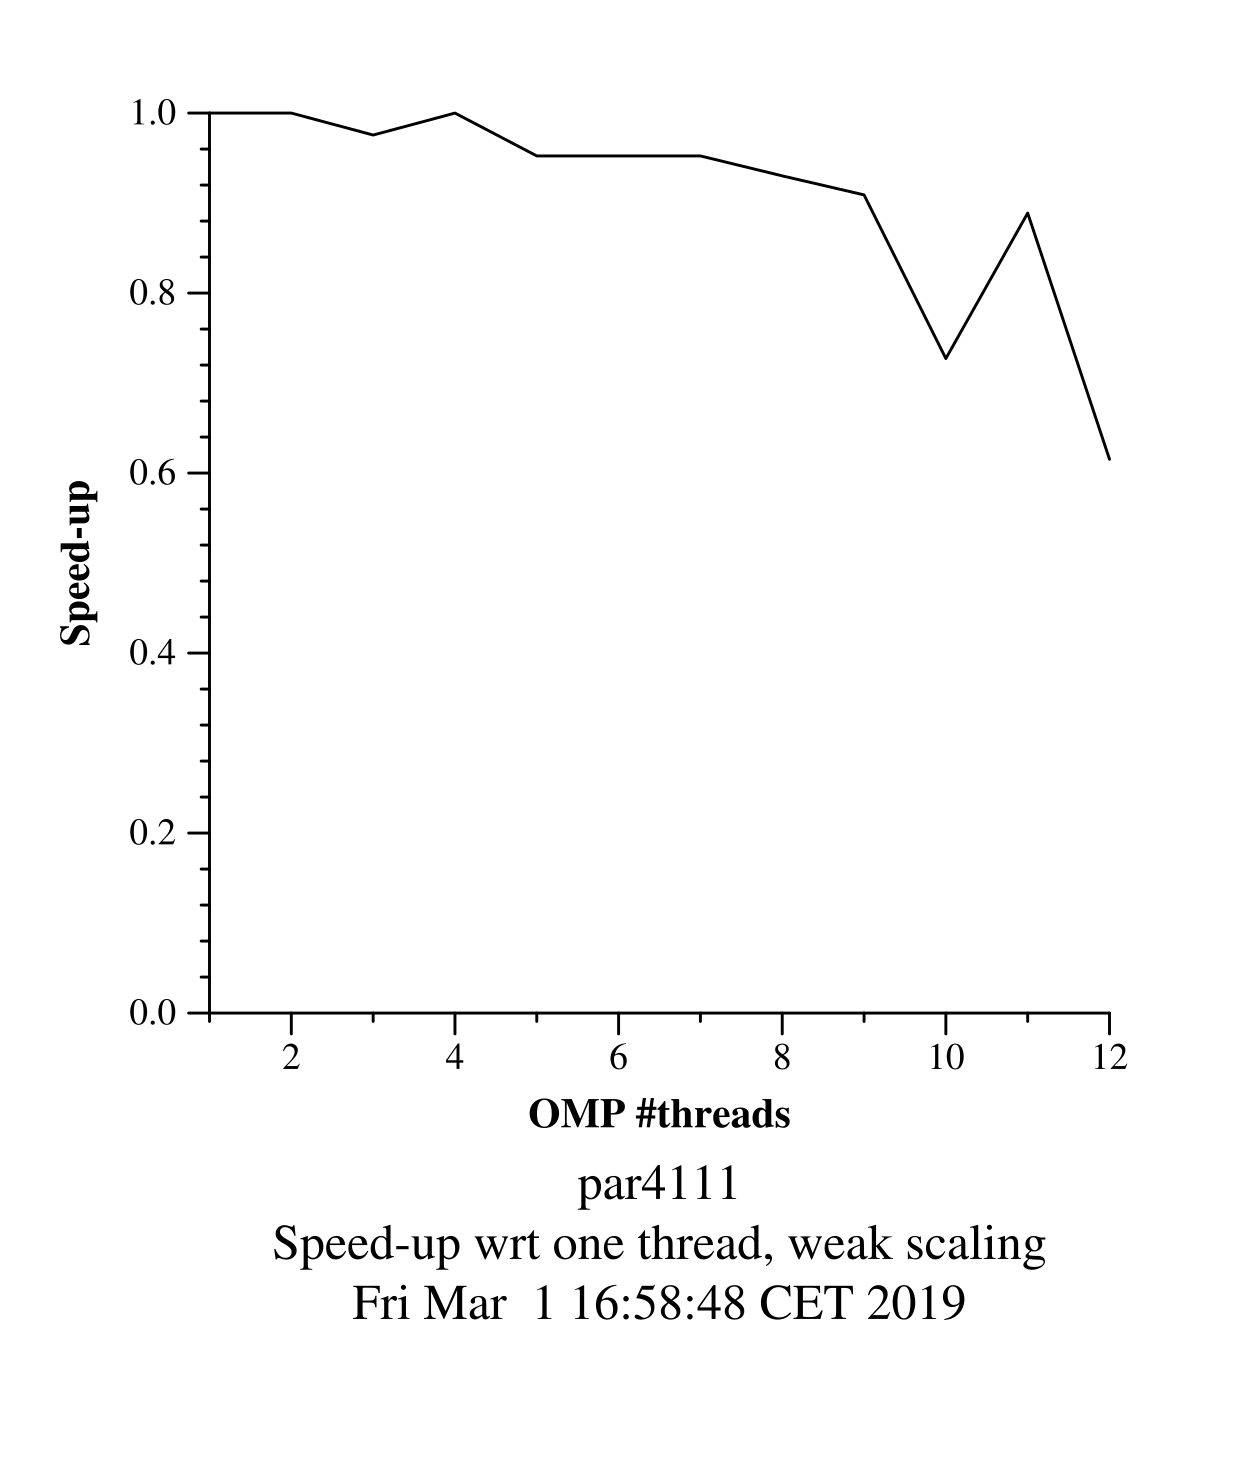
\includegraphics[scale=0.15]{images/pi_omp-100000000-1-12-3-weak-boada-3.png}
 \caption{ \textit{pi\_omp} with weak scalability by Boada-3}
  \label{fig:pi_weak_ompboada3}
\end{figure}

\bigskip
\paragraph{Boada 5:}
For Boada 5 we observe a similar behaviour, but this time speed-up goes over 1, meaning the problem size could be increased faster if we wanted to keep speed-up steady. In the end, however, overhead still counters the extra processors and speed-up goes down at around 10-12 threads.
\begin{figure}[H]
\centering
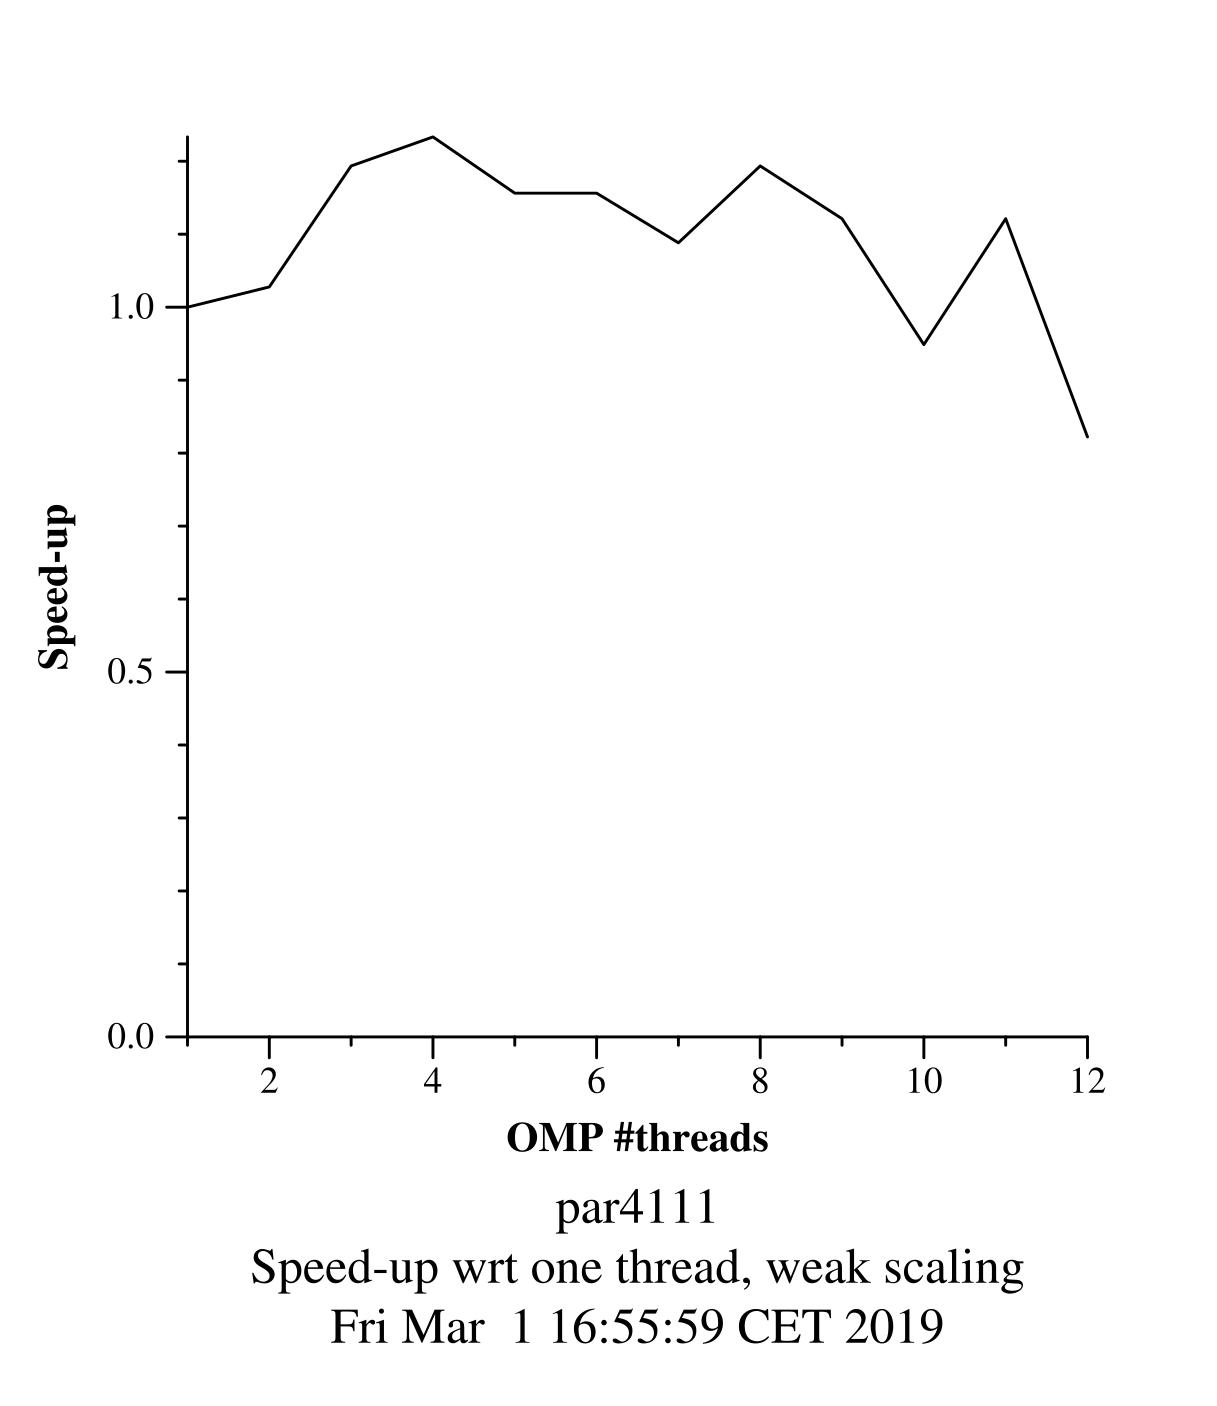
\includegraphics[scale=0.15]{images/pi_omp-100000000-1-12-3-weak-boada-5.png}
 \caption{ \textit{pi\_omp} with weak scalability by Boada-5}
  \label{fig:pi_weak_ompboada5}
\end{figure}

\bigskip
\paragraph{Boada 6 to 8:}
With Boada 6 to 8 we encounter the same situation as in strong scalability. There is no clear sign of overhead occuring in Figure \ref{fig:pi_weak_ompboada6}. Again, it would happen if we kept increasing the number of threads assuming the program could use them all, but up to 12 threads there is not a real downside of parallelizing the program too much.
\begin{figure}[H]
\centering
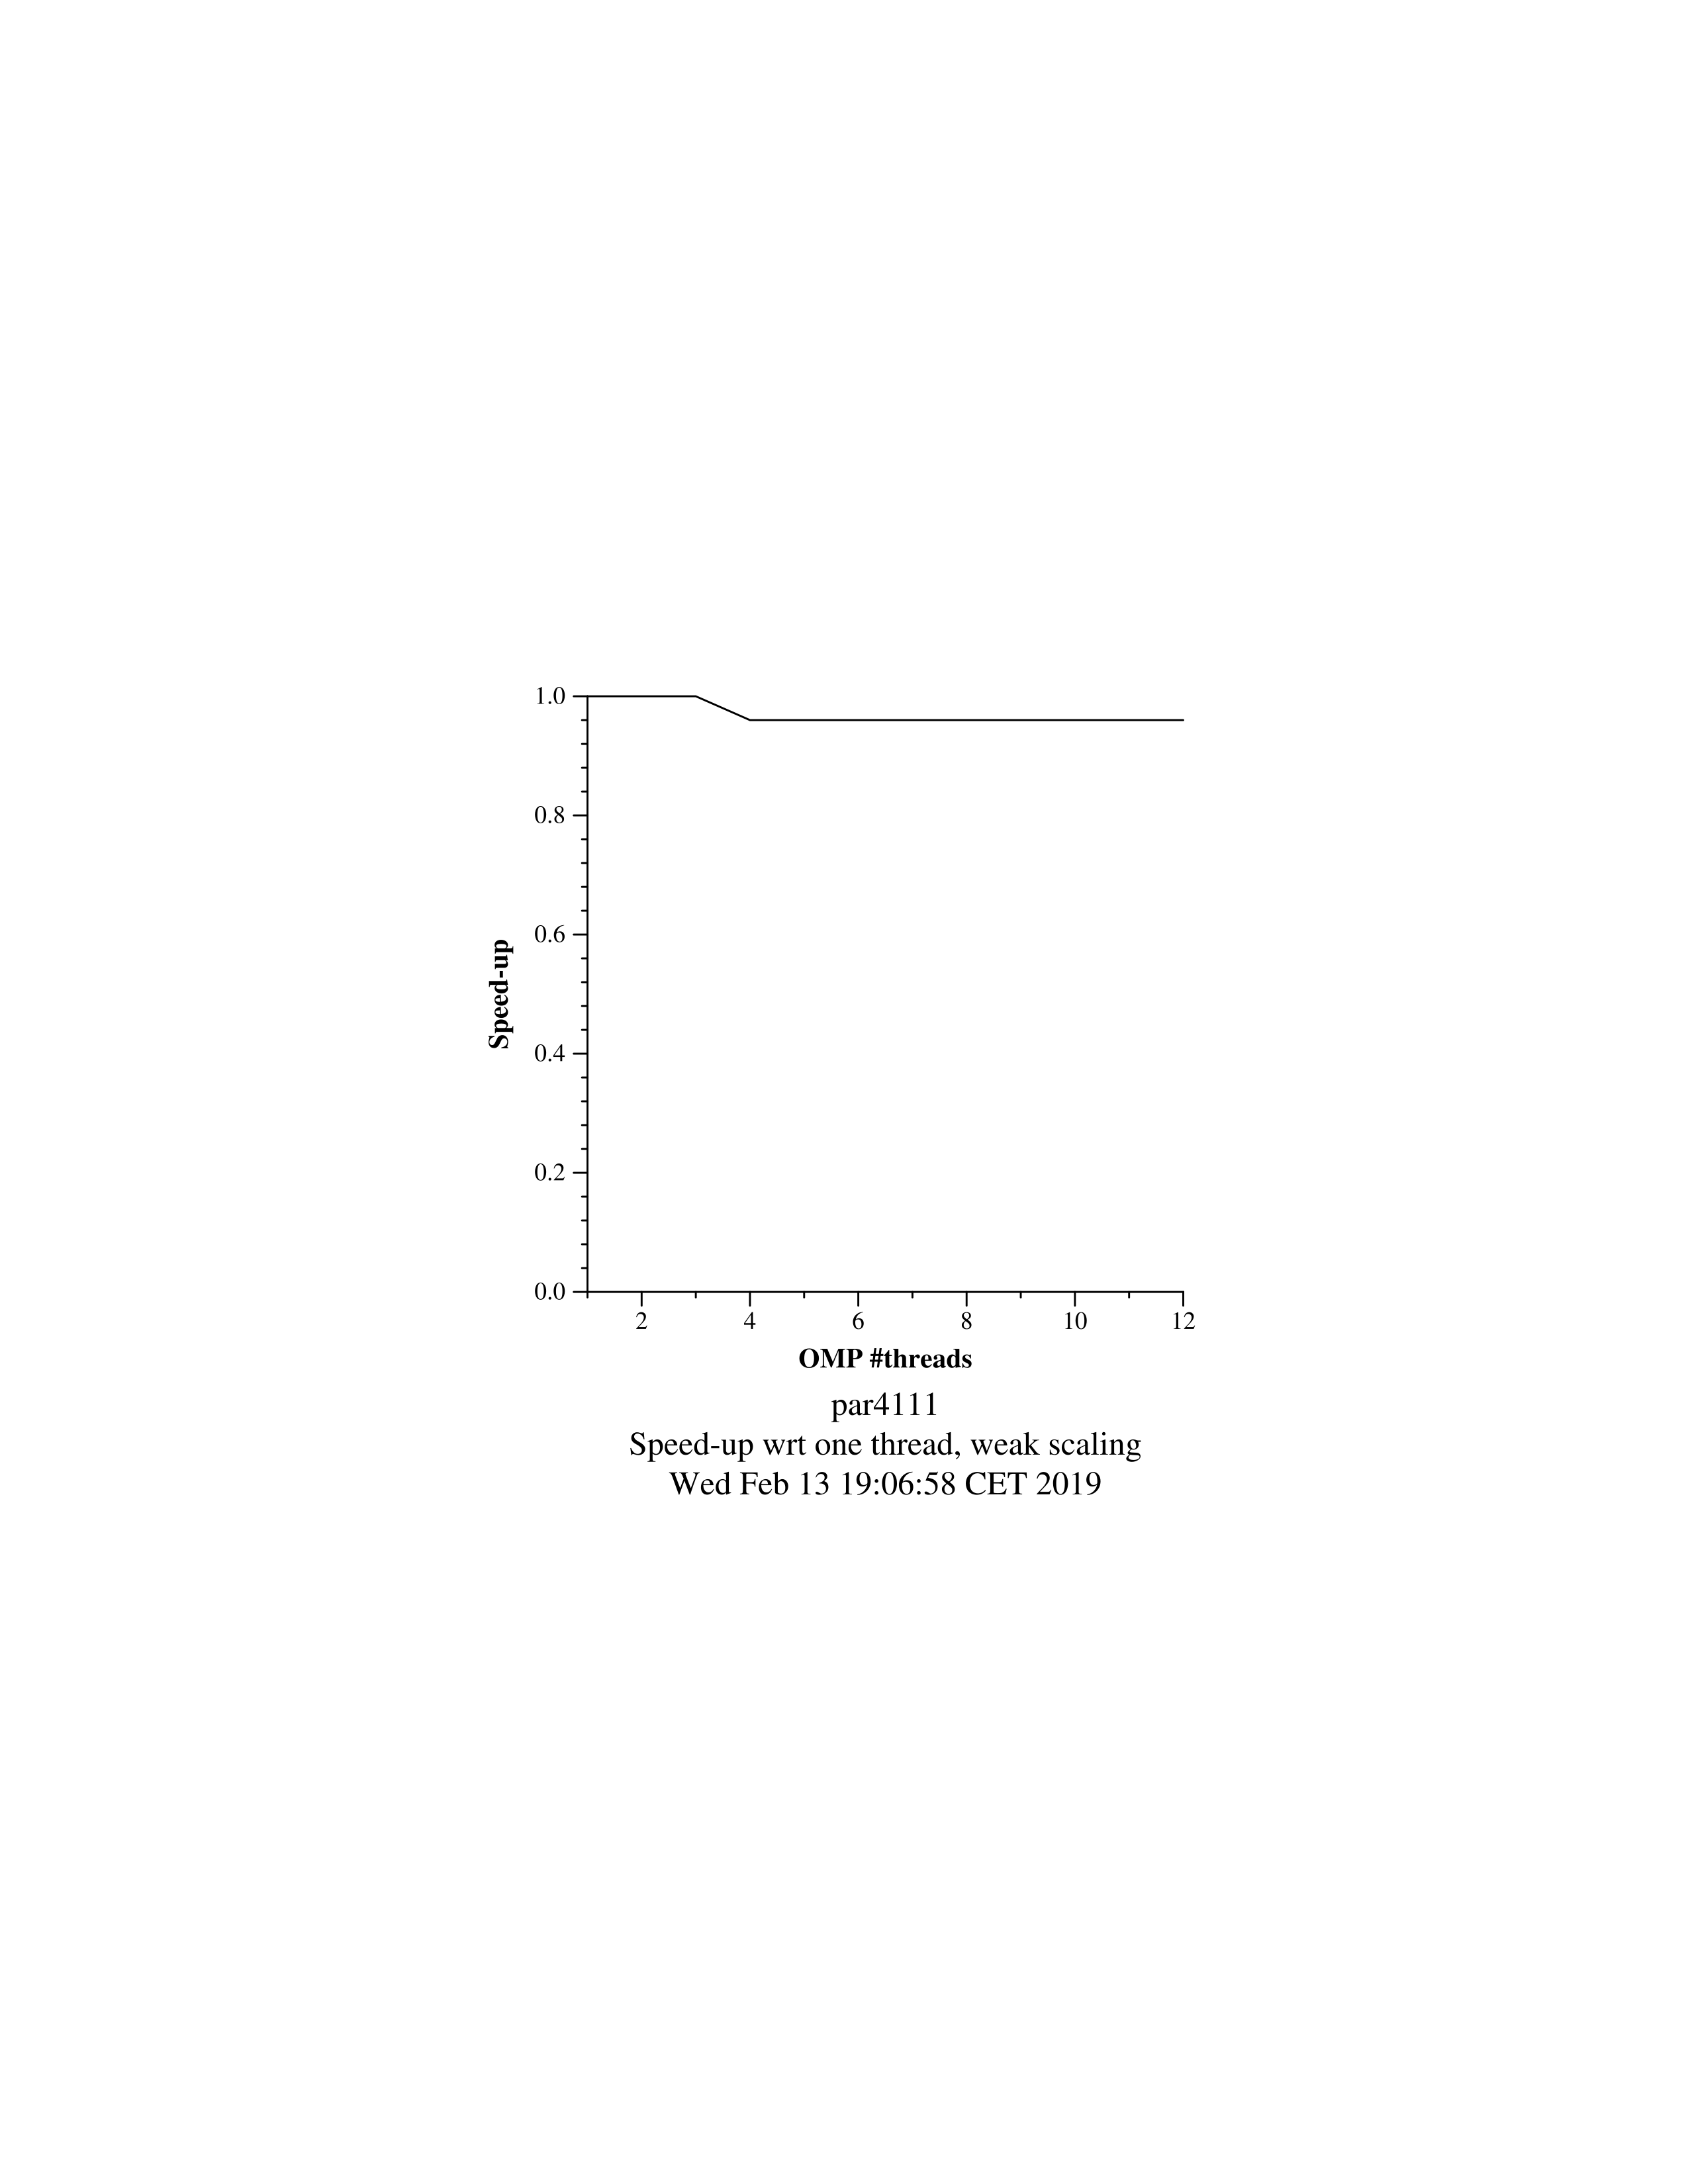
\includegraphics[scale=0.15]{images/pi_omp-100000000-1-12-3-weak-boada-6.png}
 \caption{ \textit{pi\_omp} with weak scalability by Boada-6}
  \label{fig:pi_weak_ompboada6}
\end{figure}

\section{Systematically analysing task decompositions with Tareador}
\subsection{Introduction}
The objective of this laboratory is learn how to use \textit{Tareador}, an environment to analyse the potential parallelilsm that can be obtained when a certain task decomposition is applied to a code. We will introduce how it works and we will experiment and analyse decomposition with a sequential code called 3DFFT.
\subsection{Analysis of task decompositions for 3DFFT}

After seeing the basic features in \textit{Tareador} we can now proceed to explore new tasks decompositions for a piece of code. Down below we will incrementally generate five new task decompositions and the potential parallelism ($T_1 / T_\infty$) from the task dependence graph generated by \textit{Tareador}. 
\\
To obtain $T_\infty$ we will assume that each instruction takes one time unit to execute and simulate the execution of the graph with a large number of processors.

Once we have created those tasks, we can visualize the dependency graph using \textit{Tareador}. Each node of the graph represents a task: diferents shapes and colours are used to identify task instances and each one is labeled with a task instance number and some important information like the number of instructions. Also the size of the shape reflects in some way its granularity.

\begin{figure}[H]
\centering  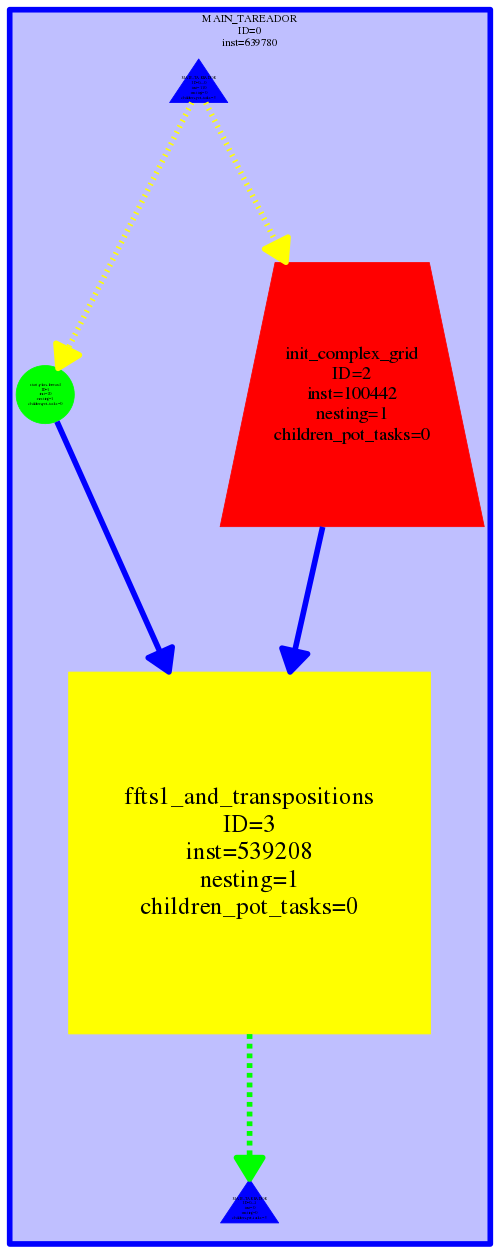
\includegraphics[width=.8\linewidth, height=14cm, width=6cm]{images/dependency_graph0.png}
  \caption{Dependency graph for the original version.}
  \label{fig:Depencency0}
\centering
\end{figure}



\subsubsection{Version 1}

The first version consists in replacing the task named \texttt{ffts1\_and\_transpositions} with a sequence of finer grained tasks, one for each function invocation inside it. The modified code is the following: 
\\
\begin{lstlisting}
...
    tareador_start_task("0");
    ffts1_planes(p1d, in_fftw);
    tareador_end_task("0");

    tareador_start_task("1");
    transpose_xy_planes(tmp_fftw, in_fftw);
    tareador_end_task("1");

    tareador_start_task("2");
    ffts1_planes(p1d, tmp_fftw);
    tareador_end_task("2");

    tareador_start_task("3");	
    transpose_zx_planes(in_fftw, tmp_fftw);
    tareador_end_task("3");
    
    tareador_start_task("4");
    ffts1_planes(p1d, in_fftw);
    tareador_end_task("4");

    tareador_start_task("5");
    transpose_zx_planes(tmp_fftw, in_fftw);
    tareador_end_task("5");

    tareador_start_task("6");
    transpose_xy_planes(in_fftw, tmp_fftw);
    tareador_end_task("6");
\end{lstlisting}

Once we have created all these tasks, we have to execute the script \textit{./run-tareador.sh VERSION1} and visualize the task dependence graph, see Figure \ref{fig:Dependency1st}. As we can see comparing it to the original graph; the shape that was associated to \texttt{ffts1\_and\_transpositions} has now been divided into several other shapes which represents more granularity. 

\begin{figure}[H]
\centering  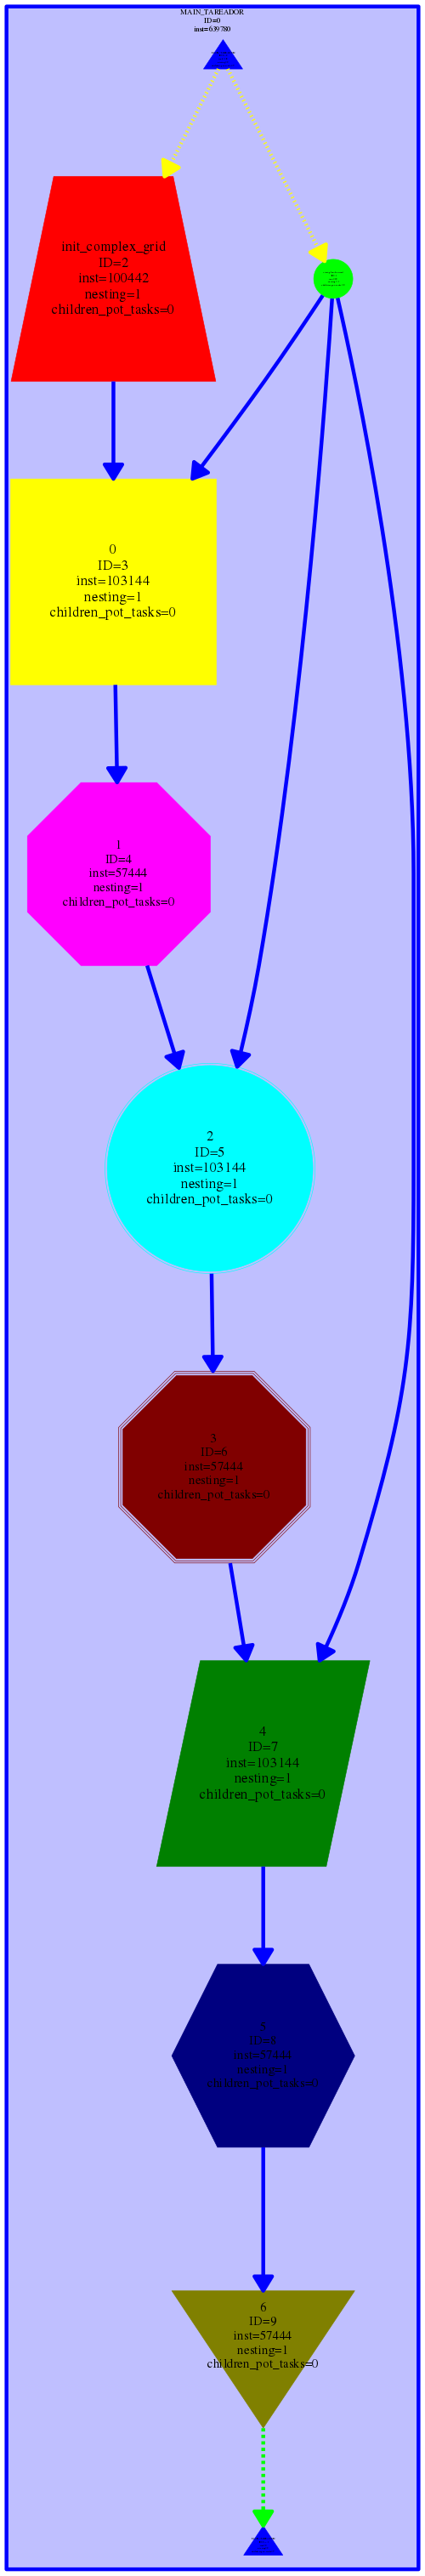
\includegraphics[width=\linewidth, height=22cm, width=4cm]{images/dependency_graph1.png}
  \caption{Dependency graph for the first version.}
  \label{fig:Dependency1st}
\end{figure}



\subsubsection{Version 2}

The second version, starting from the first one, consists in replacing the definition of tasks associated to function invocations \texttt{ffts1\_planes} with fine-grained tasks defined inside the function body and associated to individual iterations of the k loop. The changes that have been made in the code for this version are the following ones: 
\\ \medskip
\begin{lstlisting}

void ffts1_planes(fftwf_plan p1d, fftwf_complex in_fftw[][N][N]) {
    int k,j;

    for (k=0; k<N; k++) {
     tareador_start_task("ffts1_planes_loop_k");
     for (j=0; j<N; j++) {
       fftwf_execute_dft( p1d, (fftwf_complex *)in_fftw[k][j][0], (fftwf_complex *)in_fftw[k][j][0]);
     }
     tareador_end_task("ffts1_planes_loop_k");
    }
}


int main(){
...
    tareador_start_task("1");
    transpose_xy_planes(tmp_fftw, in_fftw);
    tareador_end_task("1");

    ffts1_planes(p1d, tmp_fftw);

    tareador_start_task("3");	
    transpose_zx_planes(in_fftw, tmp_fftw);
    tareador_end_task("3");

    ffts1_planes(p1d, in_fftw);

    tareador_start_task("5");
    transpose_zx_planes(tmp_fftw, in_fftw);
    tareador_end_task("5");

    tareador_start_task("6");
    transpose_xy_planes(in_fftw, tmp_fftw);
    tareador_end_task("6");
...
}

\end{lstlisting}

As we can see in the outputed dependency graph given by the \textit{Tareador}, it has changed and there are several more shapes. The task that previously was \texttt{ffts1\_planes} has been divided into several more. 
\begin{figure}[H]
\centering  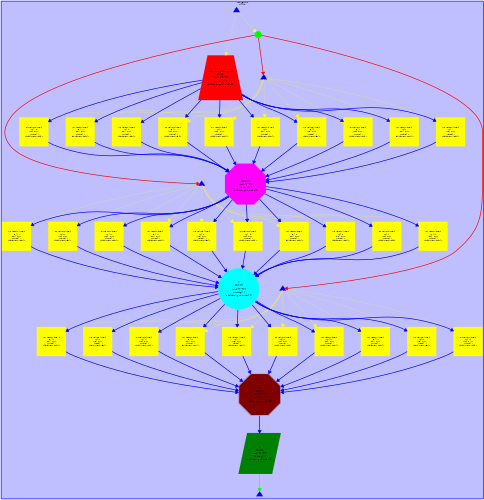
\includegraphics[width=\linewidth , height=13cm, width=13cm ]{images/dependency_graph2.png}
  \caption{Dependency graph for the second version.}
  \label{fig:Depencency2nd}
\end{figure}


\subsubsection{Version 3}
The third version, starting from the second one, consists in replacing the definition of tasks associated to function invocations \texttt{transpose\_xy\_planes} and \texttt{transpose\_zx\_planes} with fine-grained tasks inside the corresponding body functions and associated to individual iterations of the k loop, similarly as it was made in the second version. 
\begin{lstlisting}
void transpose_xy_planes(fftwf_complex  tmp_fftw[][N][N], fftwf_complex in_fftw[][N][N]) {
    int k,j,i;

    for (k=0; k<N; k++) {
     tareador_start_task("transpose_xy_planes_loop_k");
     for (j=0; j<N; j++) {
       for (i=0; i<N; i++)
       {
         tmp_fftw[k][i][j][0] = in_fftw[k][j][i][0];
         tmp_fftw[k][i][j][1] = in_fftw[k][j][i][1];
       }
     }
     tareador_end_task("transpose_xy_planes_loop_k"); 
   }
}

void transpose_zx_planes(fftwf_complex in_fftw[][N][N], fftwf_complex tmp_fftw[][N][N]) {
    int k, j, i;

    for (k=0; k<N; k++) {
    tareador_start_task("transpose_zx_planes_loop_k");
    for (j=0; j<N; j++) {
      for (i=0; i<N; i++)
       {
         in_fftw[i][j][k][0] = tmp_fftw[k][j][i][0];
         in_fftw[i][j][k][1] = tmp_fftw[k][j][i][1];
       }
     }
     tareador_end_task("transpose_zx_planes_loop_k");

    }
}

int main(){
...
    tareador_start_task("init_complex_grid");
    init_complex_grid(in_fftw);
    tareador_end_task("init_complex_grid");

    STOP_COUNT_TIME("Init Complex Grid FFT3D");

    START_COUNT_TIME;

    ffts1_planes(p1d, in_fftw);
    transpose_xy_planes(tmp_fftw, in_fftw);
    ffts1_planes(p1d, tmp_fftw);
    transpose_zx_planes(in_fftw, tmp_fftw);
    ffts1_planes(p1d, in_fftw);
    transpose_zx_planes(tmp_fftw, in_fftw);
    transpose_xy_planes(in_fftw, tmp_fftw);
...
}
\end{lstlisting}

Like in the previous cases, we can now see in the dependency graph our results and the level of granularity we are getting. 

\begin{figure}[H]
\centering  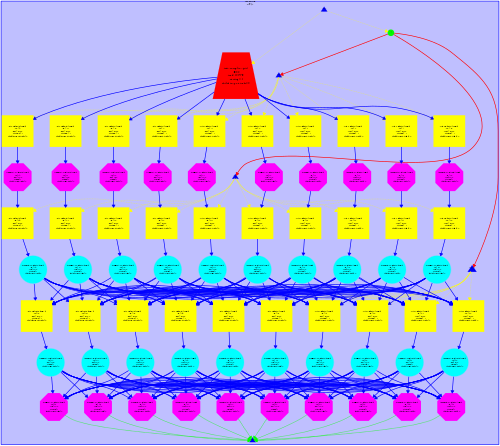
\includegraphics[width=\linewidth , height=13cm, width=13cm  ]{images/dependency_graph3.png}
  \caption{Dependency graph for the third version.}
  \label{fig:Depencency3rd}
\end{figure}

\subsubsection{Version 4}
The forth version, starting from the third one, consists in replacing the definition of tasks associated to function invocations \texttt{init\_complex\_grid}  with fine-grained tasks inside the corresponding body functions and associated to individual iterations of the k loop, like it was made in the previous version. 

\begin{lstlisting}
void init_complex_grid(fftwf_complex in_fftw[][N][N]) {
  int k,j,i;

  for (k = 0; k < N; k++) {
    tareador_start_task("transpose_init_complex_grid_loop_k");
    for (j = 0; j < N; j++) {
      for (i = 0; i < N; i++)
      {
        in_fftw[k][j][i][0] = (float) (sin(M_PI*((float)i)/64.0)+sin(M_PI*((float)i)/32.0)+sin(M_PI*((float)i/16.0)));
        in_fftw[k][j][i][1] = 0;
#if TEST
        out_fftw[k][j][i][0]= in_fftw[k][j][i][0];
        out_fftw[k][j][i][1]= in_fftw[k][j][i][1];
#endif
      }
    }
 
     tareador_end_task("transpose_init_complex_grid_loop_k"); 
 }
}
int main(){
...

    init_complex_grid(in_fftw);
    STOP_COUNT_TIME("Init Complex Grid FFT3D");

    START_COUNT_TIME;

    ffts1_planes(p1d, in_fftw);
    transpose_xy_planes(tmp_fftw, in_fftw);
    ffts1_planes(p1d, tmp_fftw);
    transpose_zx_planes(in_fftw, tmp_fftw);
    ffts1_planes(p1d, in_fftw);
    transpose_zx_planes(tmp_fftw, in_fftw);
    transpose_xy_planes(in_fftw, tmp_fftw);
...
}

\end{lstlisting}

\begin{figure}[H]
\centering  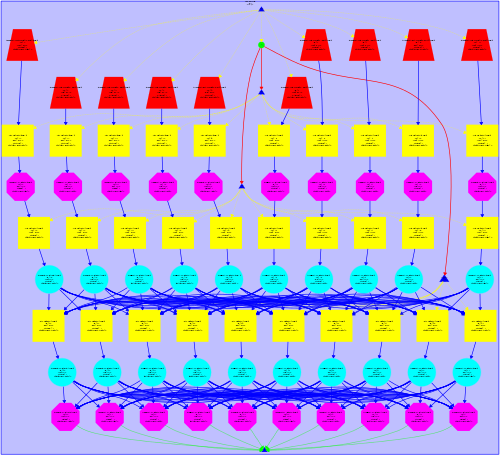
\includegraphics[width=\linewidth , height=13cm, width=13cm  ]{images/dependency_graph4.png}
  \caption{Dependency graph for the forth version.}
  \label{fig:Dependency4rth}
\end{figure}


\subsubsection{Version 5}
This is the final version and we will explore even more finer-grained tasks. In order to continue this task we observed the figure given by \textit{Tareador} that corresponds to the forth version of the code. 

As we can see in the Figure \ref{fig:Dependency4rth} the task  that has less granularity is the \textit{ffts1\_planes\_loop\_k} with 10305 instructions each. So we deepen in the code of the corresponding function and we created tasks in a loop deeper than our first approach. 
\begin{lstlisting}

void ffts1_planes(fftwf_plan p1d, fftwf_complex in_fftw[][N][N]) {
    int k,j;
    for (k=0; k<N; k++) {
     for (j=0; j<N; j++) {
       tareador_start_task("ffts1_planes_loop_j");

        fftwf_execute_dft( p1d, (fftwf_complex *)in_fftw[k][j][0], (fftwf_complex *)in_fftw[k][j][0]);
    tareador_end_task("ffts1_planes_loop_j");
         }

    }
}


\end{lstlisting}
\bigskip

\begin{figure}[H]
\centering  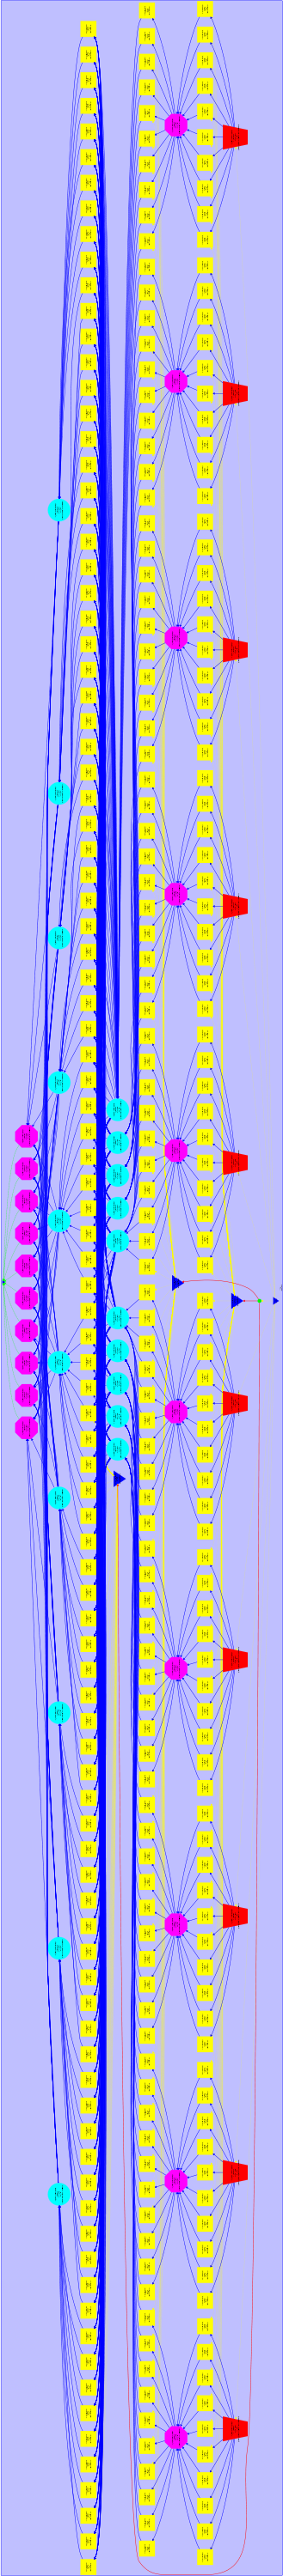
\includegraphics[width=\linewidth , height=13cm, width=4cm  ]{images/dependency_graph5.png}
  \caption{Dependency graph for the final version.}
  \label{fig:Dependency5}
\end{figure}

\subsubsection{Comparison between version 4 and version 5}


\begin{large}
\begin{center}
Time comparison (in ns) between version 4 and version 5
\end{center}
\end{large}
\begin{table}[h]
\begin{center}
Number of processors 
\end{center}
\begin{tabular}{l|l|l|l|l|l|l|}
\cline{2-7}

                         & 1           & 2           & 4           & 8          & 16         & 32         \\ \hline
\multicolumn{1}{|l|}{v4} & 639.780.001 & 320.310.001 & 165.389.001 & 91.496.001 & 64.018.001 & 64.018.001 \\ \hline
\multicolumn{1}{|l|}{v5} & 639.780.001 & 321.493.001 & 172.584.001 & 99.126.001 & 53.554.001 & 44.356.001 \\ \hline
\end{tabular}
\end{table}

\begin{figure}[H]
\centering  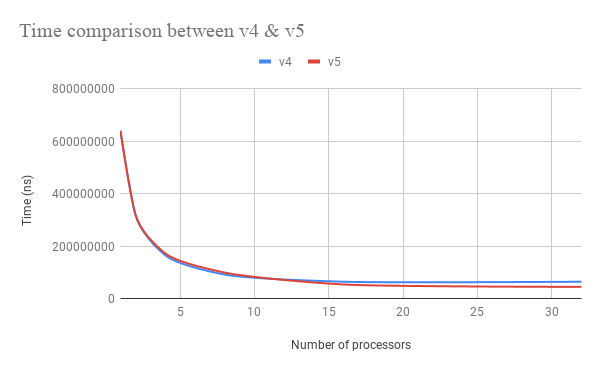
\includegraphics[width=\linewidth]{images/Time.png}
  \caption{Time comparison between v4 and v5.}
  \label{fig:PlotComparison}
\end{figure}

\begin{large}
\begin{center}
Speedup between version 4 and version 5
\end{center}
\end{large}

\begin{table}[h]
\begin{center}
Number of processors 
\end{center}
\begin{tabular}{l|l|l|l|l|l|l|}
\cline{2-7}
                              & 1 & 2              & 4              & 8              & 16            & 32            \\ \hline
\multicolumn{1}{|l|}{Speedup} & 1 & 0.99632029 & 0.95831015 & 0.92302725 & 1.1953915 & 1.4432771 \\ \hline
\end{tabular}
\end{table}


\begin{figure}[H]
\centering  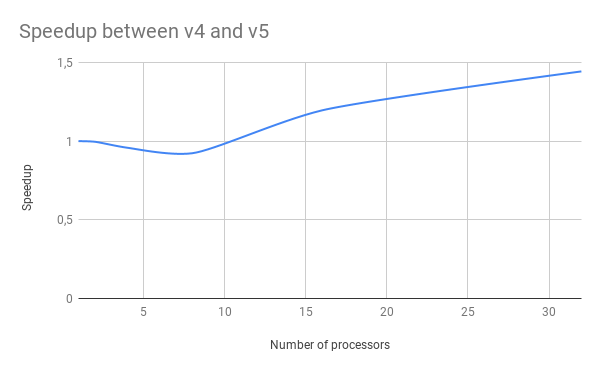
\includegraphics[width=\linewidth]{images/Speedup.png}
  \caption{Speedup between v4 and v5.}
  \label{fig:PlotComparison}
\end{figure}


From this two plots we can observe that there's a moment when it does not matter how many processors we use, we cannot improve the execution time we can get. In the case of the fourth version we can see it clearly comparing the time we get with 16 processors and the time we get with 32. \\

Moreover, there is still another interesting point we can still analyse. Even though the fifth version had more finer-grained tasks (check Figure \ref{fig:Dependency5} when we use less than 16 processors v4 gets a better time execution. That could be justified with the time is focused for making the finer-grained tasks work together because of the overhead.  

\subsubsection{Summary}
To sum up, we show a table with all the data obtained with our experiments. We can see that in all the versions excepting for the first ones, we increase the parallelism.
\\
\medskip
\begin{table}[H]
\centering
\begin{tabular}{|l|l|l|l|}
\hline
Version & $T_1 $ & $T_\infty$ & Parallelism \\ \hline
seq     & 639,780,001 ns   & 639,707,001 ns    &        1.00011411474     \\ \hline
v1      &  639,780,001 ns  & 639,707,001 ns  &         1.00011411474      \\ \hline
v2      & 639,780,001 ns   & 361,190,001 ns   &      1.77131149597      \\ \hline
v3      & 639,780,001 ns   & 154,354,001 ns &         4.14488770524    \\ \hline
v4      & 639,780,001 ns   &  64,018,001 ns   &        9.99375161683     \\ \hline
v5      &639,780,001 ns     & 38,224,001 ns  &        16.7376513254    \\ \hline
\end{tabular}
\end{table}

\section{Understanding the parallel execution}
In this final section we have used \textit{Paraver} and several of its configurations to be able to understand better differently parallelized versions of the \textit{3dfft\_omp} program

\subsection{Initial version}
The first version we have tried is the one given to us, which is already parallelized partially. The for loop inside the init\_complex\_grid function is not parallelized. As seen in the table below, this will cause the parallel fraction to not be as high as the following versions. Nonetheless, there is still a good improvement from using 8 threads instead of 1, execution time has been halved. In fact, due to the low parallel fraction of this version, ideal speed-up with infinite processors is 2.12 while speed-up with 8 is 2.07, which is pretty close to the limit. In Figure \ref{fig:3ddftStrongPlot} we can appreciate how 8 threads have actually the best performance, and if we keep increasing the number of threads then overhead starts to make speed-up decay.

\begin{figure}[H]
\centering  
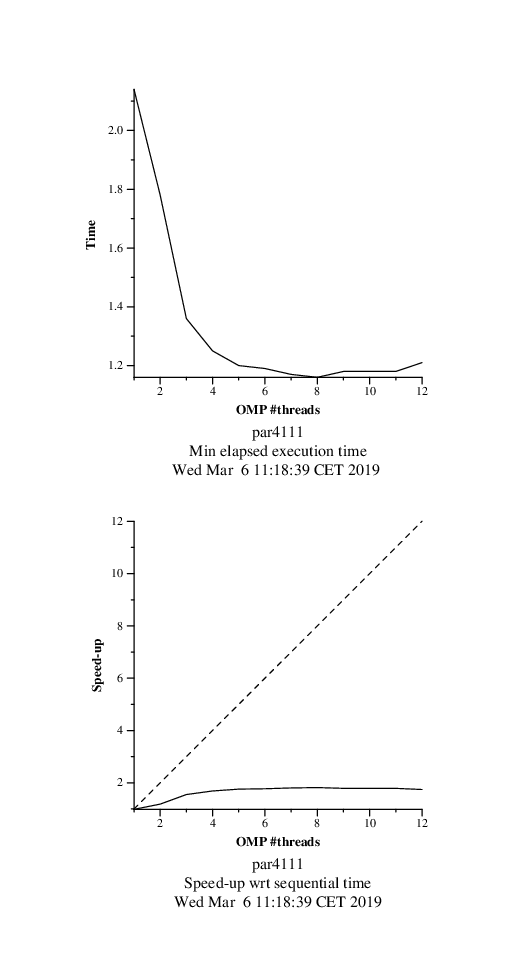
\includegraphics[scale=0.5]{images/3dfft/strongPlot.PNG}
  \caption{Strong scalability plot of the first version of 3dfft\_omp.c}
  \label{fig:3ddftStrongPlot}
\end{figure}

\bigskip
Following are screen captures of \textit{Paraver} state config, timeline and parallel functions durations config (the latter to get $T{par}$):

\bigskip

\begin{figure}[H]
\centering  
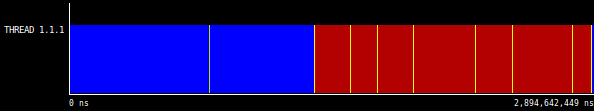
\includegraphics[scale=0.5]{images/3dfft/1threadTimeline.PNG}
    \caption{Timeline of the first version of 3dfft\_omp.c with 1 thread}
\end{figure}

\begin{figure}[H]
\centering  
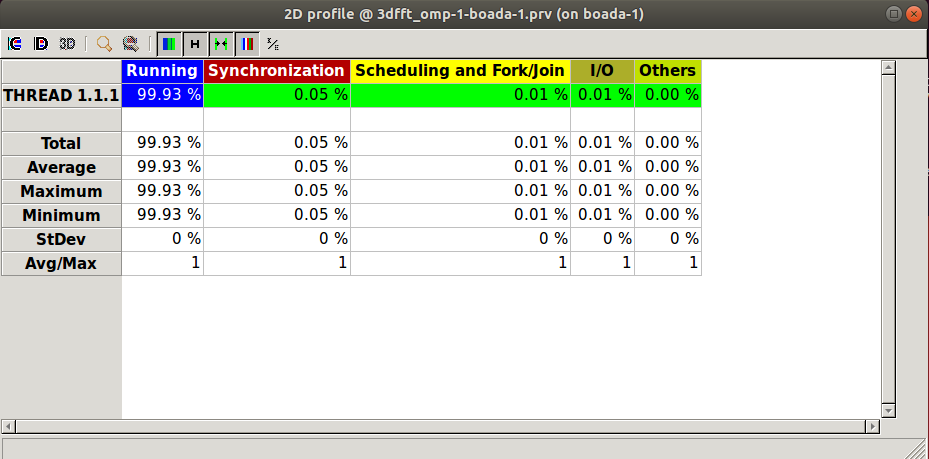
\includegraphics[scale=0.5]{images/3dfft/1threadPercentage.PNG}
    \caption{State config with (\% time) of the first version of 3dfft\_omp.c with 1 thread}
\end{figure}

\begin{figure}[H]
\centering  
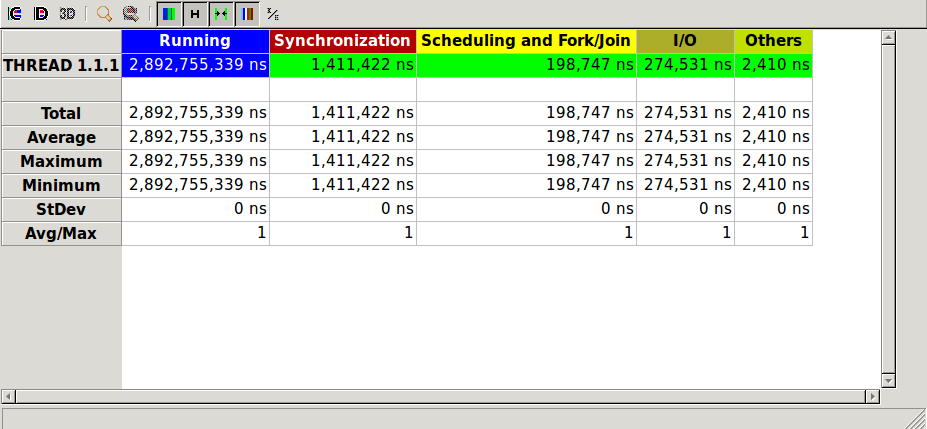
\includegraphics[scale=0.5]{images/3dfft/1thread.PNG}
    \caption{State config with (time) of the first version of 3dfft\_omp.c with 1 thread}
\end{figure}
    

\begin{figure}[H]
\centering  
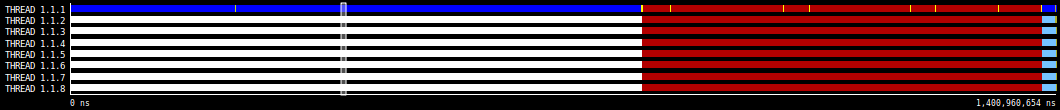
\includegraphics[scale=0.5]{images/3dfft/8threadsTimeline.PNG}
    \caption{Timeline of the first version of 3dfft\_omp.c with 8 threads}
\end{figure}
    
\begin{figure}[H]
\centering  
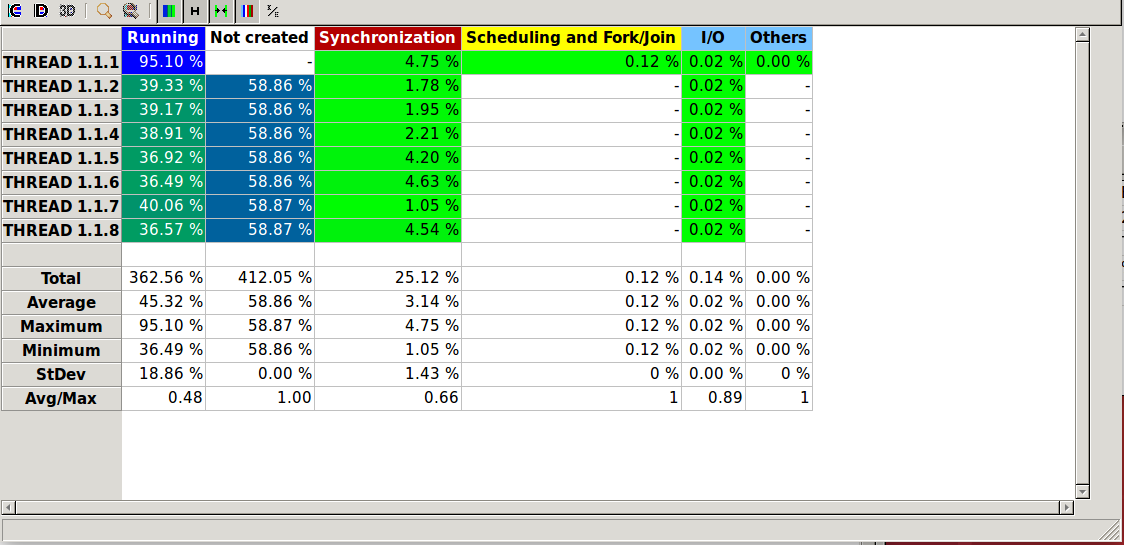
\includegraphics[scale=0.5]{images/3dfft/8threadsPercentage.PNG}
    \caption{State config with (\% time) of the first version of 3dfft\_omp.c with 8 threads}
\end{figure}

\begin{figure}[H]
\centering  
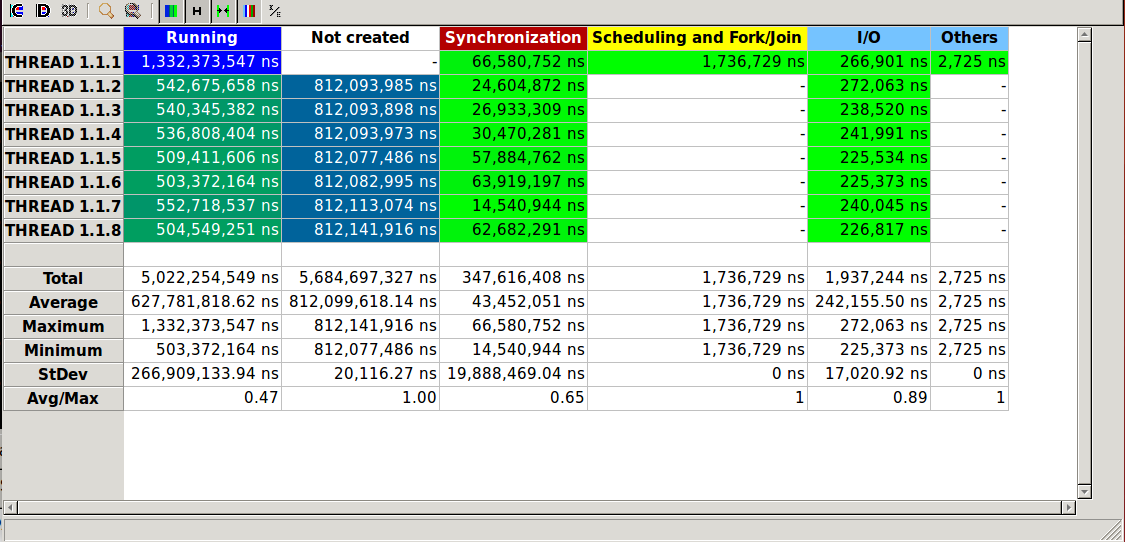
\includegraphics[scale=0.5]{images/3dfft/8threads.PNG}
    \caption{State config with (time) of the first version of 3dfft\_omp.c with 8 threads}
\end{figure}

\begin{figure}[H]
\centering  
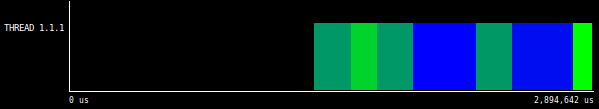
\includegraphics[scale=0.5]{images/3dfft/parallelFunction.PNG}
    \caption{Parallel function duration config with of the first version of 3dfft\_omp.c with 1 thread. Painted parts represent $T{par}$.}
\end{figure}
        

\subsection{Improving $\phi$}
In this section we uncommented a line inside the init\_complex\_grid function to allow parallelization in its for loop. This incrased the parallel fraction notably (see results in table below and Figure \ref{fig:parFunc2}). It went from 0.53 to 0.85, which allowed speed-up with 8 threads to go from 2.07 to 2.55, a good result but far from what is ideally possible. Thanks to this change, ideal speed-up with infinite processors has gone up to 6.67. The problem again is that there is too much overhead from 9 threads on, as seen in Figure \ref{fig:imp3ddftStrongPlot}.

\begin{figure}[H]
\centering  
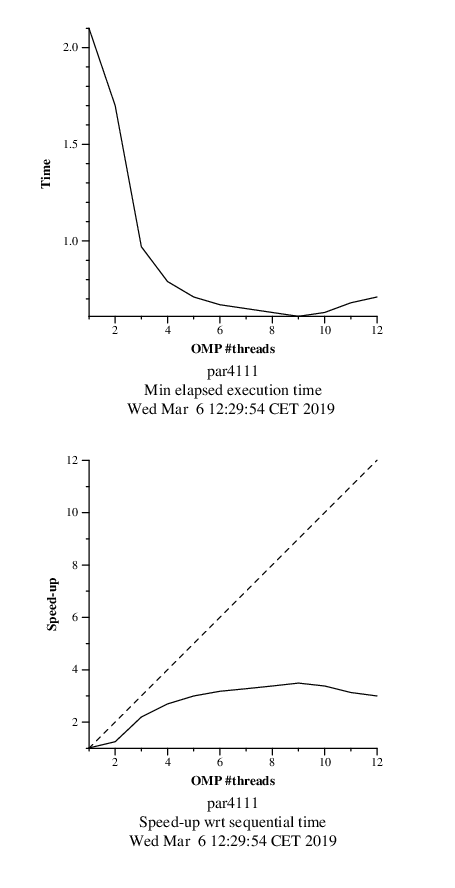
\includegraphics[scale=0.5]{images/improved_3dfft/strongPlot.PNG}
  \caption{Strong scalability plot of the second version of 3dfft\_omp.c}
  \label{fig:imp3ddftStrongPlot}
\end{figure}

\bigskip
Following are screen captures of \textit{Paraver} state config, timeline and parallel functions durations config (the latter to get $T{par}$):

\bigskip

\begin{figure}[H]
\centering  
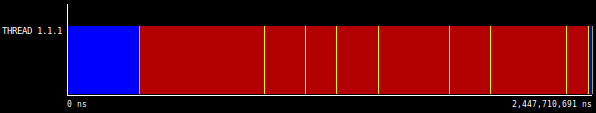
\includegraphics[scale=0.5]{images/improved_3dfft/1threadTimeline.PNG}
    \caption{Timeline of the second version of 3dfft\_omp.c with 1 thread}
\end{figure}

\begin{figure}[H]
\centering  
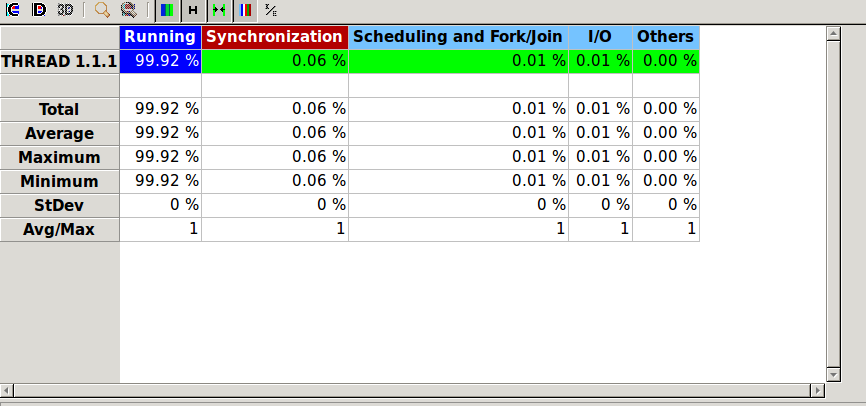
\includegraphics[scale=0.5]{images/improved_3dfft/1threadPercentage.PNG}
    \caption{State config with (\% time) of the second version of 3dfft\_omp.c with 1 thread}
\end{figure}

\begin{figure}[H]
\centering  
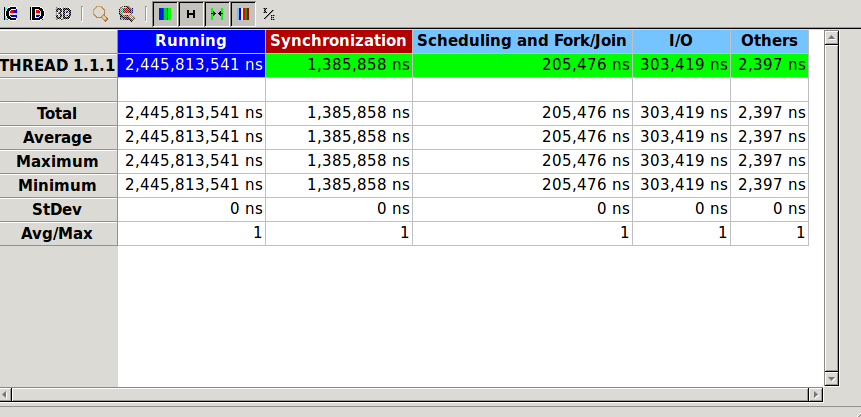
\includegraphics[scale=0.5]{images/improved_3dfft/1thread.PNG}
    \caption{State config with (time) of the second version of 3dfft\_omp.c with 1 thread}
\end{figure}
    

\begin{figure}[H]
\centering  
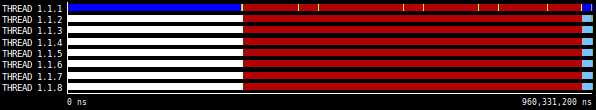
\includegraphics[scale=0.5]{images/improved_3dfft/8threadsTimeline.PNG}
    \caption{Timeline of the second version of 3dfft\_omp.c with 8 threads}
\end{figure}
    
\begin{figure}[H]
\centering  
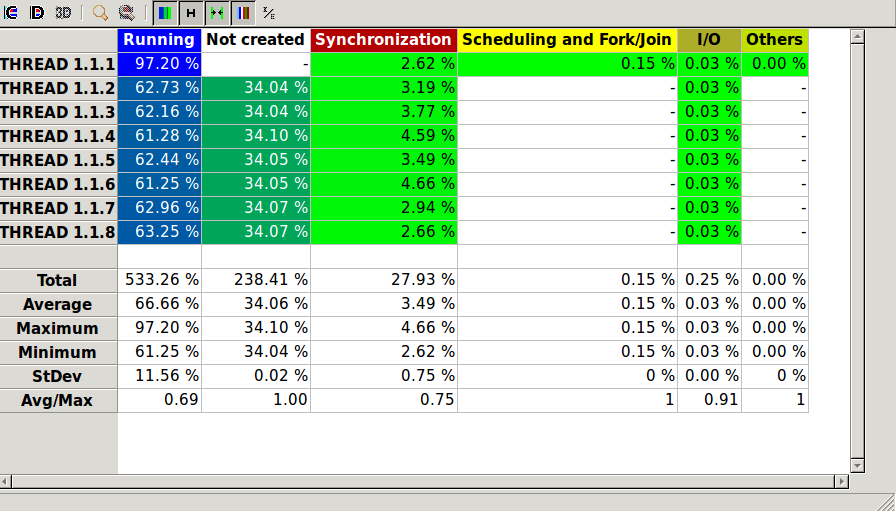
\includegraphics[scale=0.5]{images/improved_3dfft/8threadsPercentage.PNG}
    \caption{State config with (\% time) of the second version of 3dfft\_omp.c with 8 threads}
\end{figure}

\begin{figure}[H]
\centering  
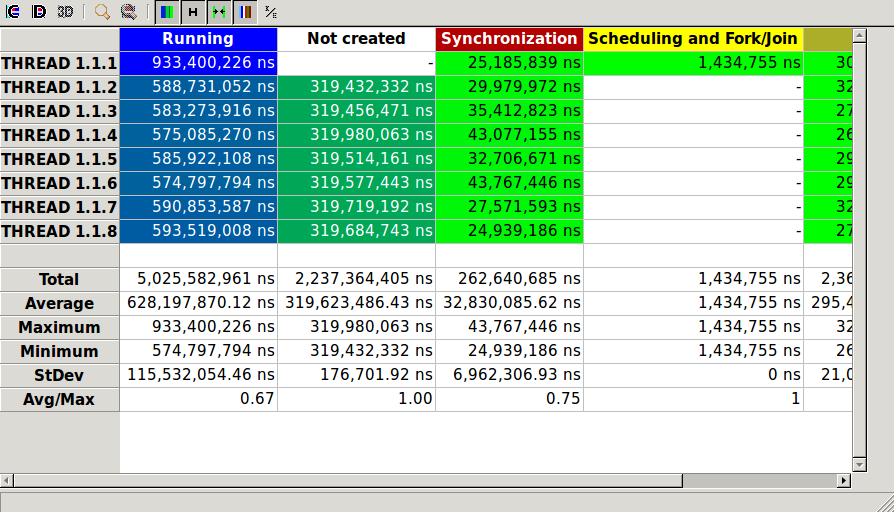
\includegraphics[scale=0.5]{images/improved_3dfft/8threads.PNG}
    \caption{State config with (time) of the second version of 3dfft\_omp.c with 8 threads}
\end{figure}

\begin{figure}[H]
\centering  
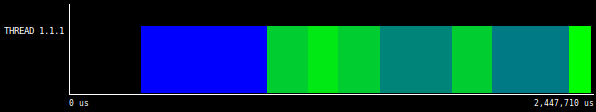
\includegraphics[scale=0.5]{images/improved_3dfft/parallelFunction.PNG}
    \caption{Parallel function duration config with of the second version of 3dfft\_omp.c with 1 thread. Painted parts represent $T{par}$.}
    \label{fig:parFunc2}
\end{figure}


\subsection{Reducing parallelisation overheads}
In this last version, we moved all the "\#pragma omp for" lines one line above to include the upper for loop. This increases the granularity of tasks and should reduce overhead caused by parallelisation. \\
As shown in the table below, it has indeed worked. Speed-up for 8 threads has gone from 2.55 to 2.72, even though total execution time has been increased both for 1 and 8 threads. So even if execution time has increased, the main goal has been achieved, which was to reduce overhead with respect to version 2.

\begin{figure}[H]
\centering  
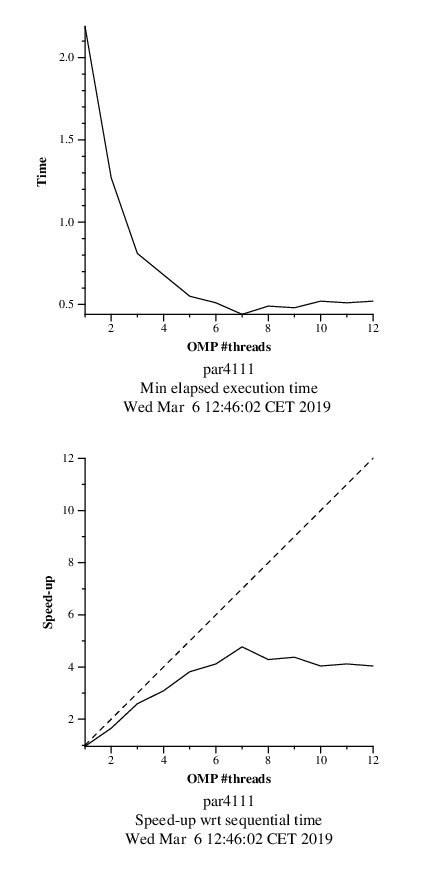
\includegraphics[scale=0.5]{images/megaImproved_3dfft/strongPlot.PNG}
  \caption{Strong scalability plot of the third version of 3dfft\_omp.c}
  \label{fig:imp23ddftStrongPlot}
\end{figure}

\bigskip
Following are screen captures of \textit{Paraver} state config, timeline and parallel functions durations config (the latter to get $T{par}$):

\bigskip

\begin{figure}[H]
\centering  
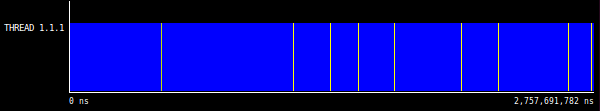
\includegraphics[scale=0.5]{images/megaImproved_3dfft/1threadTimeline.PNG}
    \caption{Timeline of the third version of 3dfft\_omp.c with 1 thread}
\end{figure}

\begin{figure}[H]
\centering  
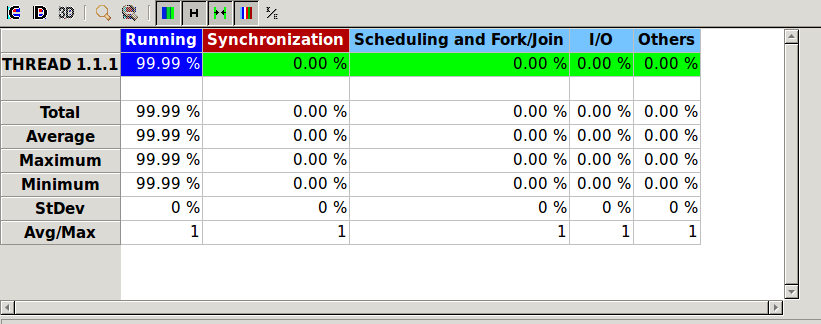
\includegraphics[scale=0.5]{images/megaImproved_3dfft/1threadPercentage.PNG}
    \caption{State config with (\% time) of the third version of 3dfft\_omp.c with 1 thread}
\end{figure}

\begin{figure}[H]
\centering  
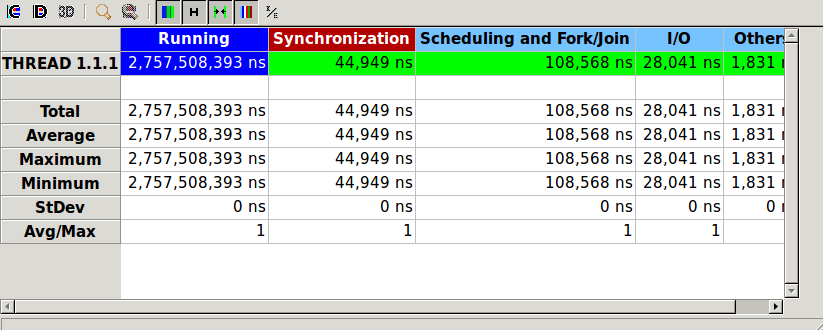
\includegraphics[scale=0.5]{images/megaImproved_3dfft/1thread.PNG}
    \caption{State config with (time) of the third version of 3dfft\_omp.c with 1 thread}
\end{figure}
    

\begin{figure}[H]
\centering  
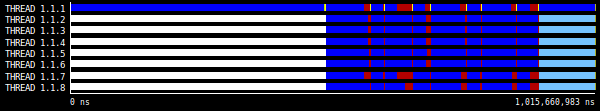
\includegraphics[scale=0.5]{images/megaImproved_3dfft/8threadsTimeline.PNG}
    \caption{Timeline of the third version of 3dfft\_omp.c with 8 threads}
\end{figure}
    
\begin{figure}[H]
\centering  
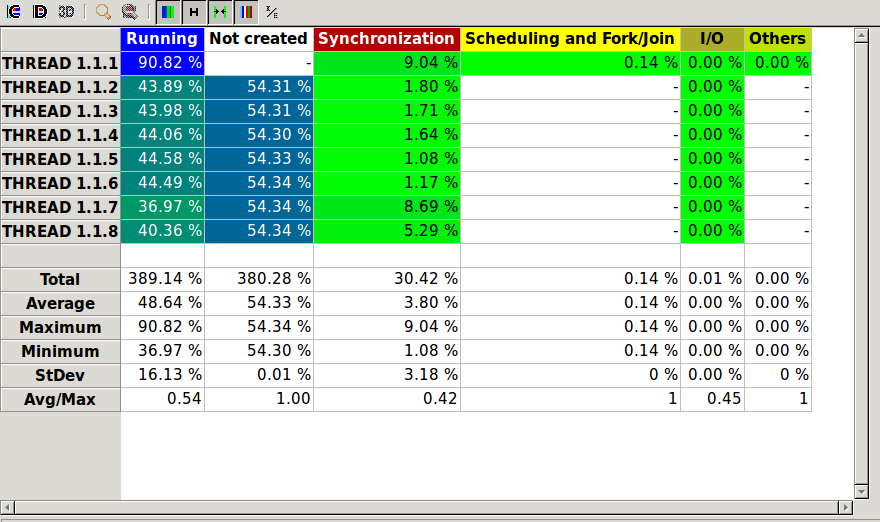
\includegraphics[scale=0.5]{images/megaImproved_3dfft/8threadsPercentage.PNG}
    \caption{State config with (\% time) of the third version of 3dfft\_omp.c with 8 threads}
\end{figure}

\begin{figure}[H]
\centering  
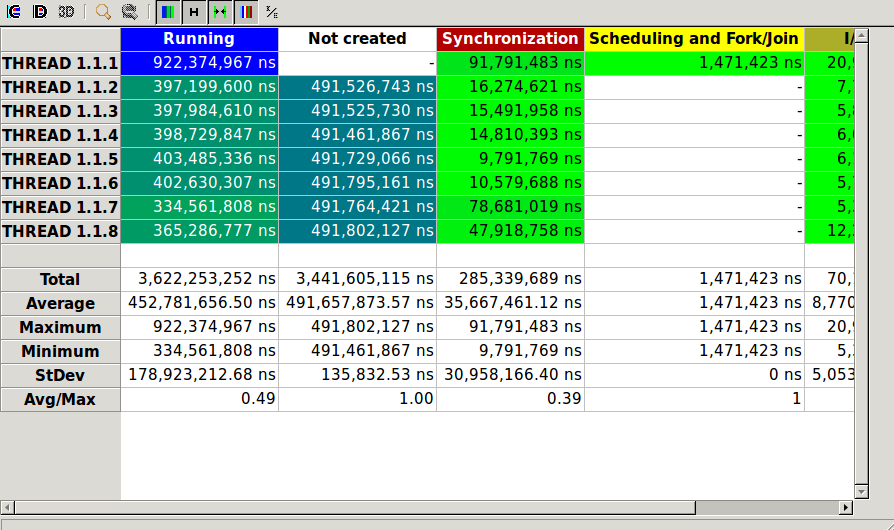
\includegraphics[scale=0.5]{images/megaImproved_3dfft/8threads.PNG}
    \caption{State config with (time) of the third version of 3dfft\_omp.c with 8 threads}
\end{figure}

\begin{figure}[H]
\centering  
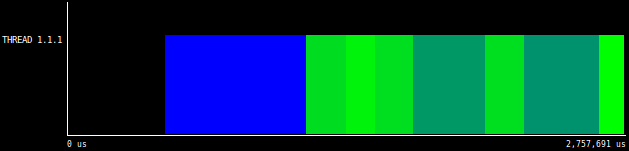
\includegraphics[scale=0.5]{images/megaImproved_3dfft/parallelFunction.PNG}
    \caption{Parallel function duration config with of the third version of 3dfft\_omp.c with 1 thread. Painted parts represent $T{par}$.}
    \label{fig:parFunc3}
\end{figure}






\subsection{Final results}

The results obtained are in the following table:
\textit{Note that $S{8}$ has been calculated using $T1$ and $T8$, and $T1$ has been exctracted from executing the parallelised version 3dfft\_omp with 1 thread. For this reason, speed-up is different from the ones on the strong scalability plots, which use the sequential version of 3dfft to calculate.}

\bigskip

\begin{table}[H]
\begin{tabular}{|l|l|l|l|l|l|}
\hline \textbf{Version} & $\phi $ & $S_\infty$ & $T_1$ & $T_8$ & $S_8$ \\ \hline
initial version in \textit{3dfft\_omp.c} & 0.53 & 2.12 & 2895 ms & 1400 ms & 2.07 \\ \hline
new version with improved $\phi$ & 0.85 & 6.67 & 2448 ms & 960 ms & 2.55 \\ \hline
final version with reduced parallelisation overhead & 0.82 & 5.56 & 2758 ms & 1015 ms & 2.72 \\ \hline

\end{tabular}
\end{table}

\bigskip

\begin{center}
$\phi = T_{par} / (T_{seq} + T_{par}) $ \\
$S_\infty = 1 / (1 - \phi) $
\end{center}

\bigskip

3dfft: \\
Tpar = 1523 ms \\
Tseq = 1372 ms \\

3dfft improving parallel fraction: \\
Tpar = 2087 ms \\
Tseq = 361 ms \\

3dfft reducing overhead: \\
Tpar = 2258 ms \\
Tseq = 500 ms \\
%he pensat que maybe podriem treure les conclusions ss\section{Conclusions}

\end{document}
